\documentclass[11pt, a4paper]{article}
\usepackage[utf8]{inputenc}
\usepackage[margin=.7in]{geometry}
\usepackage{listings}
\usepackage{setspace}
\usepackage{xcolor}
\usepackage{titlesec}
\usepackage{enumitem}
\usepackage{amssymb}
\usepackage{amsmath}
\usepackage{bm}
\usepackage{multicol}
\usepackage{graphicx}
\graphicspath{{./Figures/}}
\usepackage{color}
\usepackage{hyperref}
\hypersetup{
	colorlinks=true,
	linkcolor=blue,
	urlcolor=blue,
}
\titleformat*{\section}{\LARGE\bfseries\filcenter}
\titleformat*{\subsection}{\Large\bfseries}
\titleformat*{\subsubsection}{\large\bfseries}
\definecolor{codegreen}{rgb}{0,0.5,0}
\definecolor{codegray}{rgb}{0.5,0.5,0.5}
\definecolor{codered}{rgb}{0.78,0,0}
\definecolor{codepurple}{rgb}{0.58,0,0.68}
\definecolor{backcolour}{rgb}{0.95,0.95,0.92}
\lstdefinestyle{Pythonstyle}{
	language = Python,
    backgroundcolor=\color{backcolour},   
    commentstyle=\color{gray},
    keywordstyle=\color{codegreen},
    numberstyle=\tiny\color{codegray},
    stringstyle=\color{codered},
    basicstyle=\ttfamily\footnotesize,
    breakatwhitespace=false,         
    breaklines=true,                 
    captionpos=b,                    
    keepspaces=true,                 
    numbers=left,                    
    numbersep=5pt,                  
    showspaces=false,                
    showstringspaces=false,
    showtabs=false,                  
    tabsize=2,
    morekeywords = {as},
    keywordstyle = \color{codegreen}
}
\lstset{style=Pythonstyle}

\begin{document}
	\begin{titlepage}
		\begin{center} \Huge \textbf{Machine Learning in Python} \end{center}
		\tableofcontents
		\newpage
	\end{titlepage}
%%%% PAGE 1 %%%%

	\begin{spacing}{1.1}
	\section{Six Step Machine Learning Framework}
	There are six steps that we can take during the iterative process that cover the idea of \textit{Data Modeling}: \vspace*{1mm}\\
	\hspace*{2mm} 1) Problem Definition - Is it Supervised or Unsupervised? Classification or Regression? \\
	\hspace*{2mm} 2) Data - What kind of data? Structured (csv/spreadsheets) or Unstructured (images/audio)?\\
	\hspace*{2mm} 3) Evaluation - How accurate do we need the model to be? \\
	\hspace*{2mm} 4) Features - What variables of the data can be used to help our model? \\
	\hspace*{2mm} 5) Modeling - Determine the right model based on the problem defined earlier. \\
	\hspace*{2mm} 6) Experimentation - How can we improve the model? What can we try next?
	\subsection{Step 1: Problem Definition}
	In this step, we ask ourselves "what problem are we trying to solve?". However, machine learning isn't always the optimal solution. Sometimes we must consider if a simple hand-coded instruction based system will solve our problem faster. The first task in this step is to match our problem to one of the main types of problems, which include the following. \vspace*{1mm} \\
	\textbf{Supervised Learning} uses data and labels in a machine learning algorithm in order to predict an answer. The main types of supervised learning are: \\
	\hspace*{2mm} - \textbf{Classification} : Determine which class a data point belongs two. Can be both binary (two options) \hspace*{34mm} or multi-class (more than two). \\
	\hspace*{2mm} - \textbf{Regression} : Used to predict a \textit{continuous} number. \vspace*{2mm} \\
	\textbf{Unsupervised Learning} has data but no labels. It uses this data to find patterns and classify them into groups (clusters) than can be used to find an answer to the proposed questions. This method is called \textit{Clustering}, putting groups of data together based on similarities, which can be used for things such as recommendation engines. \vspace*{2mm} \\
	\textbf{Transfer Learning} takes machine learning models that already exists and fine tunes it in order to address the problem at hand. \vspace*{2mm} \\
	\textbf{Reinforcement Learning} rewards the model for doing well or punishes it for doing poorly. For example, keeping a score and rewarding +1 when the model is correct and punishing with -1 when the model is wrong will teach the model to make choices that will maximize this `score'.
	\subsection{Step 2: Data}
	Data comes mainly in two different types: structured and unstructured. \textbf{Structured data} contains rows and columns with all of the samples in the columns being in a similar format. \textbf{Unstructured data} could be things such as images, videos, or audio files. \vspace*{2mm} \\
	Within these two data types, there is \textit{static} and \textit{streaming} data types. \textbf{Static data} is data that does not change over time (often in csv files) which can be all contained in one file separated by commas. \textbf{Streaming data} is data that is constantly changed over time (ex: news headlines effect on stock prices).\vspace*{2mm}\\
	A common data science workflow consists of: reading in static data from a csv file into a Jupyter notebook, exploring data and performing data analysis with pandas, using matplotlib to visualize any patterns/trends in the data, and finally using a machine learning model from scikit to predict using patterns. \newpage
%%%% PAGE 2 %%%%

	\subsection{Step 3: Evaluation}
	All models are used to find insights about the future, but an \textbf{evaluation metric} is a measure of how well an algorithm is at predicting the future. In this step, we want to find what percent accuracy defines success for our model. For example, if we are classifying medical records to determine heart disease diagnosis we may want our model to be over 99\% accurate. \vspace*{2mm} \\
	We use different \textbf{metrics} in order to classify the accuracy of our model based on its type: \\
	\hspace*{2mm} - Classification : We use accuracy, precision, and recall. \\
	\hspace*{2mm} - Regression : Mean absolute error (MAE), mean square error (MSE), root mean squared error (RMSE). \\
	\hspace*{2mm} - Recommendation : We use precision at K.
	\subsection{Step 4: Features}
	Features is another word for different forms of data. This could be things such as columns (feature variables) that are used to predict a new feature (target variable). \vspace*{1mm} \\ 
	Features can be both \textbf{numerical} (number value) and \textbf{categorical} (string, Boolean, etc.), while the user can create a new feature, called a \textbf{derived feature} by using existing ones. \vspace*{2mm} \\
	An important note is that features work best within a machine learning algorithm if many of the samples have it (not many missing values in the column). \textbf{Feature coverage} is how many samples have different features (ideally we want every sample to have the same features with minimal missing values).	
	\subsection{Step 5: Modeling}
	Modeling can be split into 3 different parts: choosing/training a model, tuning a model, and model comparison. However, before we do this, we must \textbf{split the data} into 3 different sets to use in each of these parts: \\
	\hspace*{2mm} - Training set : Part 1, data used to train the model (70\% - 80\%). \\
	\hspace*{2mm} - Validation set : Part 2, data used to tune/improve the model (10\% - 15\%). \\
	\hspace*{2mm} - Test set : Part 3, data used to test the accuracy of our model (10\% - 15\%). \vspace*{2mm} \\
	We feed our model the training set to set up a baseline, then we input the validation set to see if we can improve the model (\textit{model tuning}), and finally we check the results with the test set (validate our model is accurate). Be sure that the model never sees the validation/test split while training because this will throw off the true accuracy of the model. \vspace*{1mm} \\	
	\textbf{Generalization} is the ability for a machine learning model to perform well on data it hasn't seen before. However, we must be cautious not to let the validation set be the same as the test set (this can lead to memorization and no real learning for the model). \\~\\
	In part 1 of modeling, we will \textbf{chose the model} to use for the current problem. When working with \textit{structured data}, decision trees like Random Forests and Gradient Boost are the best choices. When working with \textit{unstructured data} we typically chose Deep Learning, Neural Networks, or Transfer Learning. \vspace*{1.5mm} \\ 
	After choosing a model, we want to begin to train it (the main goal is to line up the inputs and outputs). We do this by using feature variables (x) to predict target variables (y). Another goal is to minimize time between experiments (one possible way is to use a small amount of the training set to begin with if it is a large dataset). We must consider if an increase in accuracy is worth the increase in time to run. \\~\\
	In part 2 of modeling, we will \textbf{tune the model} to try and improve our model. Using the validation set, we adjust \textit{hyperparameter} based on the model we chose. For example, increasing trees in a Random Forest or the number of layers in a Neural Network. \newpage
%%%% PAGE 3 %%%%

	\noindent In part 3 of modeling, we \textbf{compare models} using the test data to see how it works in real world applications. A good model will yield similar results on all 3 sets of data (possibly a slight decline from training to test set). If the training set performance is a much higher percent than the test set, then we have \textbf{underfitting}. If the test set performance is higher than the training set performance, then we have \textbf{overfitting}. \vspace*{2mm} \\
	One of the main causes for overfitting is \textit{data leakage}, which happens when some of your test data leaks into the training data. For example, this is similar to seeing the final exam before taking it (memorization). We must make sure to properly use the correct data set for the modeling step. \vspace*{2mm} \\
	One of the main causes for underfitting is \textit{data mismatch}, which happens when the data your testing on is different than the data you are testing on. This could be caused by having different features in both of the sets. \vspace*{2mm} \\
	Some fixes for underfitting include: more advanced models, increase hyperparameters, reduce amount of features, or longer training. Some fixes for overfitting include: collecting more data or trying a less advanced models. \\
	
	\section{Pandas: Data Analysis}
	\subsection{Series, Data Frames, and CSVs}
	\textbf{Series} are 1-D objects that are created by passing a list into a pd.Series( ) method. \textbf{Data Frames} are 2-D objects that are created with multiple series or reading in a csv file, with the pd.DataFrame( ) or pd.read\_csv( ) method. Note that the column will be referred to with \textit{axis=1} and the row is referred to by \textit{axis=0}. Note that you can read in csv files from a URL as long as it is in a `raw' format. 
	\begin{lstlisting}
	import pandas as pd
	
	cars = pd.Series(['BMW', 'Toyota', 'Honda'])
	colors = pd.Series(['Red', 'Blue', 'White'])
	
	car_data = pd.DataFrame({'Car Make': cars, 'Color': colors})
	
	car_sales = pd.read_csv('car-sales.csv') \end{lstlisting} \vspace*{1mm} 
	After altering an imported Data Frame or creating a new one, we can \textbf{export} it as a csv file. The file will save in the current directory (folder) that the project is in. Note that you must pass the parameter \textit{index=False} so that it does not export the index as a column (causes duplicate index columns).
	\begin{lstlisting}
	car_sales.to_csv('exported-car-sales.csv', index=False) \end{lstlisting} \vspace*{1mm} 
	\subsection{Describing Data}
	We can use the attribute \textit{.dtypes} to get information about the data types for the data frames columns. We can get a list of the column names for our data frame by using the \textit{.columns} attribute. \vspace*{1.5mm}\\
	We can use the .describe() method to get statistical information about the numeric columns. We can use the .info() method to get a general overview of the data types, columns, index range, etc. (combination of the above attributes). \newpage
%%%% PAGE 4 %%%%

	\subsection{Selecting/Viewing Data}
	We can use the \textbf{.loc[ ]} method to access rows based on index number. Note that if there are multiple rows with the same index number, it will return all of the values with that index number. \vspace*{1mm} \\
	We can use the \textbf{.iloc[ ]} method to access rows based on index position. This will always only return a single row. \vspace*{1mm} \\
	Both .loc and .iloc allow us to us slicing when accessing rows. However, .loc will gives us  up to and including the last specified row while .iloc will gives us all up to but \textit{not} including the last specified row.
	\begin{lstlisting}
	car_sales.loc[:3] # gives us rows 0, 1, 2, 3
	car_sales.iloc[:3] # gives us rows 0, 1, 2 but not 3 \end{lstlisting} \vspace*{1mm} 
	We can filter results by using \textbf{Boolean indexing} when trying to find specific column values. 
	\begin{lstlisting}
	car_sales[car_sales['Make'] == 'Toyota'] \end{lstlisting} \vspace*{1mm} 
	We can cross over two columns to get an aggregate table by using .crosstab( ) with the first parameter being the rows and the second parameter being the columns. Similarly, if we want to \textbf{compare multiple columns}, we can use the .groupby( ) method. In the below example, we can group by the `Make' column and take the mean for each numeric varaible column. 
	\begin{lstlisting}
	pd.crosstab(car_sales['Make'], car_sales['Doors']) 
	
	car_sales.groupby(['Make']).mean() \end{lstlisting} \vspace*{1mm} 
	Pandas allows us to plot numeric columns with built in methods as well. We can use \textit{.plot()} on a column in our data frame to see a line graph of the values. We can use the \textit{.hist()} method to see a histogram plot of our column values, which shows the frequency of points on our data frame column.	
	\subsection{Manipulating Data}
	Python has built in \textbf{string methods} that lets use access and manipulate string type columns in Pandas by using the \textit{.str} accessor. Note that in order to save any changes, you have to reassign the column to the original data frame. 
	\begin{lstlisting}
	car_sales['Make'] = car_sales['Make'].str.lower() \end{lstlisting} \vspace*{1mm} 
	Missing data (NaN values) can be common with data frames. We can \textbf{fill this missing values} with the .fillna( ) method and passing in a value we want to insert into all NaN values in a column. Note that we can change values in a column without having to reassign it by passing the \textit{inplace=True} parameter if the method allows us to.
	\begin{lstlisting}
	car_sales_missing = pd.read_csv('car_sales_missing_data.csv')
	
	car_sales_missing['Odometer'].fillna(car_sales_missing['Odometer'].mean(), 
	                                     inplace=True) \end{lstlisting} \vspace*{1mm} 
	We can \textbf{drop all rows with missing values} by using the .dropna( ) method. Note that we can either use reassignment or \textit{inplace=True} when using this method. 
	\begin{lstlisting}
	car_sales_missing.dropna(inplace=True) \end{lstlisting} \vspace*{1mm} 
	We can \textbf{delete columns} by using the .drop( ) method and specify the column name, axis=1, and using inplace=True. Note that this method can also be used for rows if axis=0 is specified along with the row you want to remove from the data frame. 
	\begin{lstlisting}
	car_sales_missing.drop('Total Fuel Used', inplace=True) \end{lstlisting} \newpage
%%%% PAGE 5 %%%%

	\noindent When splitting the data into training, validation, and test sets we often want to randomize the order so that the model does not memorize inputs. One way we can \textbf{shuffle data} is by using the Pandas .sample( ) method and passing the \textit{frac=1} parameter to change the original order. Note that we data frames become larger, we can use smaller sets by changing \textit{frac} to a smaller value (between 0 and 1).  
	\begin{lstlisting}
	car_sales_shuffled = car_sales.sample(frac=1) \end{lstlisting} \vspace*{1mm} 
	If we want to \textbf{reset the index} after shuffling data, we can use the .reset\_index( ) method and passing the \textit{drop=True} parameter so that it does not make a new column with the previous index values. 
	\begin{lstlisting}
	car_sales_shuffled.reset_index(drop=True) \end{lstlisting} \vspace*{1mm} 
	We can \textbf{apply functions} (NumPy or lambda) to columns with the .apply( ) method. 
	\begin{lstlisting}
	car_sales['Odometer (KM)'] = car_sales['Odometer (KM)'].apply(lambda x : x / 1.6) \end{lstlisting} \vspace*{2mm}
	
	\section{NumPy}
	\subsection{Arrays and Attributes}
	NumPy's main \textbf{datatype} is an ndarray (n-dimensional array). We can also\textbf{ create a data frame} from a NumPy array.
	\begin{lstlisting}
	import numpy as np
	
	a1 = np.array([1, 2, 3])
	a1.shape # returns (3,) 
	
	a2 = np.array([[1, 2, 3],
	               [4, 5, 6]])
	a2.ndim # returns 2 
	
	df = pd.DataFrame(a2) \end{lstlisting} \vspace*{1mm} 	
	We can use built in functions to \textbf{create arrays} filled with specified values, random values, or filled with one given value.
	\begin{lstlisting}
	ones = np.ones((2,3)) # create a 2x3 array of 1's
	
	zeros = np.zeros((2,3)) # create a 2x3 array of 0's
	
	range_arr = np.arange(0, 10, 2) # create a 1D array from 0 to 10 (inc by 2)
	
	random_arr = np.random.randint(0, 10, size=(3,5)) 
	# create 3x5 array of random ints between 0 and 10
	
	random_arr_2 = np.random.random((5,3)) # create a 5x3 array of values between 0 and 1
	
	Random_arr_3 = np.random.rand(5,3) # create 5X3 array of random values \end{lstlisting} \vspace*{1mm} 	
	When creating a random array, the values will always be different if you run the code cell again. However, we can use the \textbf{random seed} function to always create the same numbers for a given random array. This allows us to create reproducible results as well. Note that this can be any number (it doesn't matter) but you will have to run the seed call in every cell you want reproducible results in. 
	\begin{lstlisting}
	np.random.seed(6) \end{lstlisting} \newpage
%%%% PAGE 6 %%%%

	\subsection{Array Functions}
	We can perform \textbf{aggregation} on our NumPy arrays. We want to be sure that we use Python methods on Python datatypes but use NumPy's methods on NumPy arrays. For example, a list could use sum() but a NumPy array should use np.sum(). This is to optimize speed while doing calculations since NumPy uses broadcasting and C for array operations.
	\begin{lstlisting}
	large_arr = np.random.random(100000)
	
	%timeit sum(large_arr) # approx 19.9 ms per loop (526 times slower than np method)
	%timeit np.sum(large_arr) # approx 34 us (micro) per loop \end{lstlisting} \vspace*{1mm} 
	We often discuss the spread of the data we are working with. \textbf{Variance} is the measure of the average degree to which each number is different from the mean. Note that higher variance means a wider range of numbers while a lower variance is a smaller range of numbers. \textbf{Standard Deviation} is a measure of how spread out a group of numbers is from the mean (this number is just the square root of the variance). 
	\begin{lstlisting}
	high_var = np.array([1, 100, 200, 300, 4000, 5000])
	low_var = np.array([2, 4, 6, 8, 10])
	
	np.var(high_var), np.var(low_var) # (4296133.47, 8.0)
	np.std(high_var), np.std(low_var) # (2072.712, 2.828)
	
	np.mean(high_var), np.mean(low_var) # (1600.1667, 6.0) \end{lstlisting} \vspace*{1mm} 
	We can \textbf{change the shape} on a NumPy array when we need to line up our inputs into a specific shape. One way we can do this is with the .reshape( ) method to change the dimensions of our array. It will contain the same information as before but with a different shape (could be used when needing to match dimensions in order to multiply). We can use \textbf{transpose} to switch the axis and change the shape of our array. The difference is reshape allows us to create custom shapes while transpose only switches axis. 
	\begin{lstlisting}
	a2.shape # (2, 3)
	a2_reshape = a2.reshape(2, 3, 1) # change into a 3D matrix 
	
	a2_transpose = a2.T 
	a2_transpose.shape # (3, 2) \end{lstlisting} \vspace*{1mm} 
	We can perform different types of multiplication on NumPy arrays. \vspace*{2mm}\\ \textbf{Element wise}: $\begin{bmatrix} A & B \\ C & D \end{bmatrix}_{2x2}$ * $\begin{bmatrix} E & F \\ G & H \end{bmatrix}_{2x2}$ = $\begin{bmatrix} A*E & B*F \\ C*G & D*H \end{bmatrix}_{2x2}$ \vspace*{2mm} \\
	\textbf{Dot product}: $\begin{bmatrix} A & B & C \\ D & E & F \\ G & H & I \end{bmatrix}_{3x3}$ * $\begin{bmatrix} J & K \\ L & M \\ N & O \end{bmatrix}_{3x2}$ = $\begin{bmatrix} A*J + B*L + C*N & A*K + B*M + C*O \\ D*J + E*L + F*N & D*K + E*M + F*O \\ G*J + H*L + I*N & G*K + H*M + I*O \end{bmatrix}_{3x2}$ \vspace*{1mm} \\
	Note that for the dot product, the inside numbers must match (row length of first matrix must match column length of second matrix). 
	\begin{lstlisting}
	np.random.seed(0)
	
	mat1 = np.random.randint(10, size=(5,3)) # range 0-10 of 5x3 array
	mat2 = np.random.randint(10, size=(5,3)) # range 0-10 of 5x3 array
	
	np.multiply(mat1, mat2) # element wise multiplication
	
	mat1.shape, mat2.T.shape # ((5, 3), (3, 5))
	
	mat3 = np.dot(mat1, mat2.T)
	mat3.shape # (5, 5)	\end{lstlisting} \newpage
%%%% PAGE 7 %%%%

	\noindent Dot product example 
	\begin{lstlisting}
	np.random.seed(0)
	
	sales_amount = np.random.randint(20, size=(5,3)) # 5x3 matrix of sales
	
	weekly_sales = pd.DataFrame(sales_amounts,
	                            index = ['Mon','Tues','Wed','Thrs','Fri','Sat','Sun'],
	                            columns = ['Almond', 'Peanut', 'Cashew'])
	                            
	prices = np.array([10, 8, 12])     
	prices.shape # (3,) but we need (1,3)
	
	butter_prices = pd.DataFrame(prices.reshape(1,3),
	                             index = ['Price'],
	                             columns = ['Almond', 'Peanut', 'Cashew'])  
	                                                 
	butter_prices.shape, weekly_sales.shape # ((1, 3), (5, 3))
	daily_sales = butter_prices.dot(weekly_sales.T)
	# creates a 1x5 data frame with Price as row and days as columns
	
	weekly_sales['Total ($)'] = daily_sales.T # flip so it become 5x1 matrix \end{lstlisting} \vspace*{1mm} 
	\subsubsection{Sorting Arrays}
	We can sort NumPy array's in different ways. Using the np.sort( ) method will sort each row an ascending order. We can use np.argsort( ) to get an array where each index is the position in the row that the values would be sorted in.  	
	\begin{lstlisting}
	rand_arr = np.random.randint(10, size=(3,5)) 	
	
	np.argmin(a1) # index for minimum value (0)
	np.argmax(a1) # index for maximum value (2)
	
	np.argmax(rand_array, axis=0) # return the index pos for the max value in each column
	np.argmax(rand_array, axis=1) # return the index pos for the max value in each row \end{lstlisting} \vspace*{1mm} 
	\subsubsection{Turn Images into NumPy Arrays}
	We can read in images using matplotlib into a NumPy array by using the imread( ) function. It takes the pixel values (color values) and stores them in a NumPy array. 
	\begin{lstlisting}
	import matplotlib.image import imread
	
	panda = imread('images/panda.png') 
	panda.size, panda.shape # (2446500, (2330, 3500, 3)) \end{lstlisting} \vspace*{1mm} 
	Turning your data into numbers is one of the biggest steps in machine learning. Now with this array, and after training our model, we would be able to feed in the array and the model would compare numeric values to predict what it thinks the picture is using patterns in the data. \newpage
%%%% PAGE 7 %%%%

	\section{Matplotlib: Plotting and Visualizing}
	\subsection{Types of Plots}
	When graphing our plots, we want to follow the object oriented API pattern of assigning a figure and axes object to create a graph. Lets take a look at a typical workflow we would want to follow:
	\begin{lstlisting}
	import matplotlib.pyplot as plt
	
	# 1. Prepare data
	x = [1, 2, 3, 4]
	y = [11, 22, 33, 44]
	
	# 2. Setup plot (create our objects)
	fig, ax = plt.subplots(figsize=(10, 10)) # (width, height)
	
	# 3. Plot data
	ax.plot(x, y)
	
	# 4. Customize plot
	ax.set(title='Sample Plot',
	       xlabel = 'x-axis',
	       ylabel = 'y-axis')
	       
	# 5. Save and show your figure
	fig.savefig('sample-plot.png) \end{lstlisting} \vspace*{1mm}
	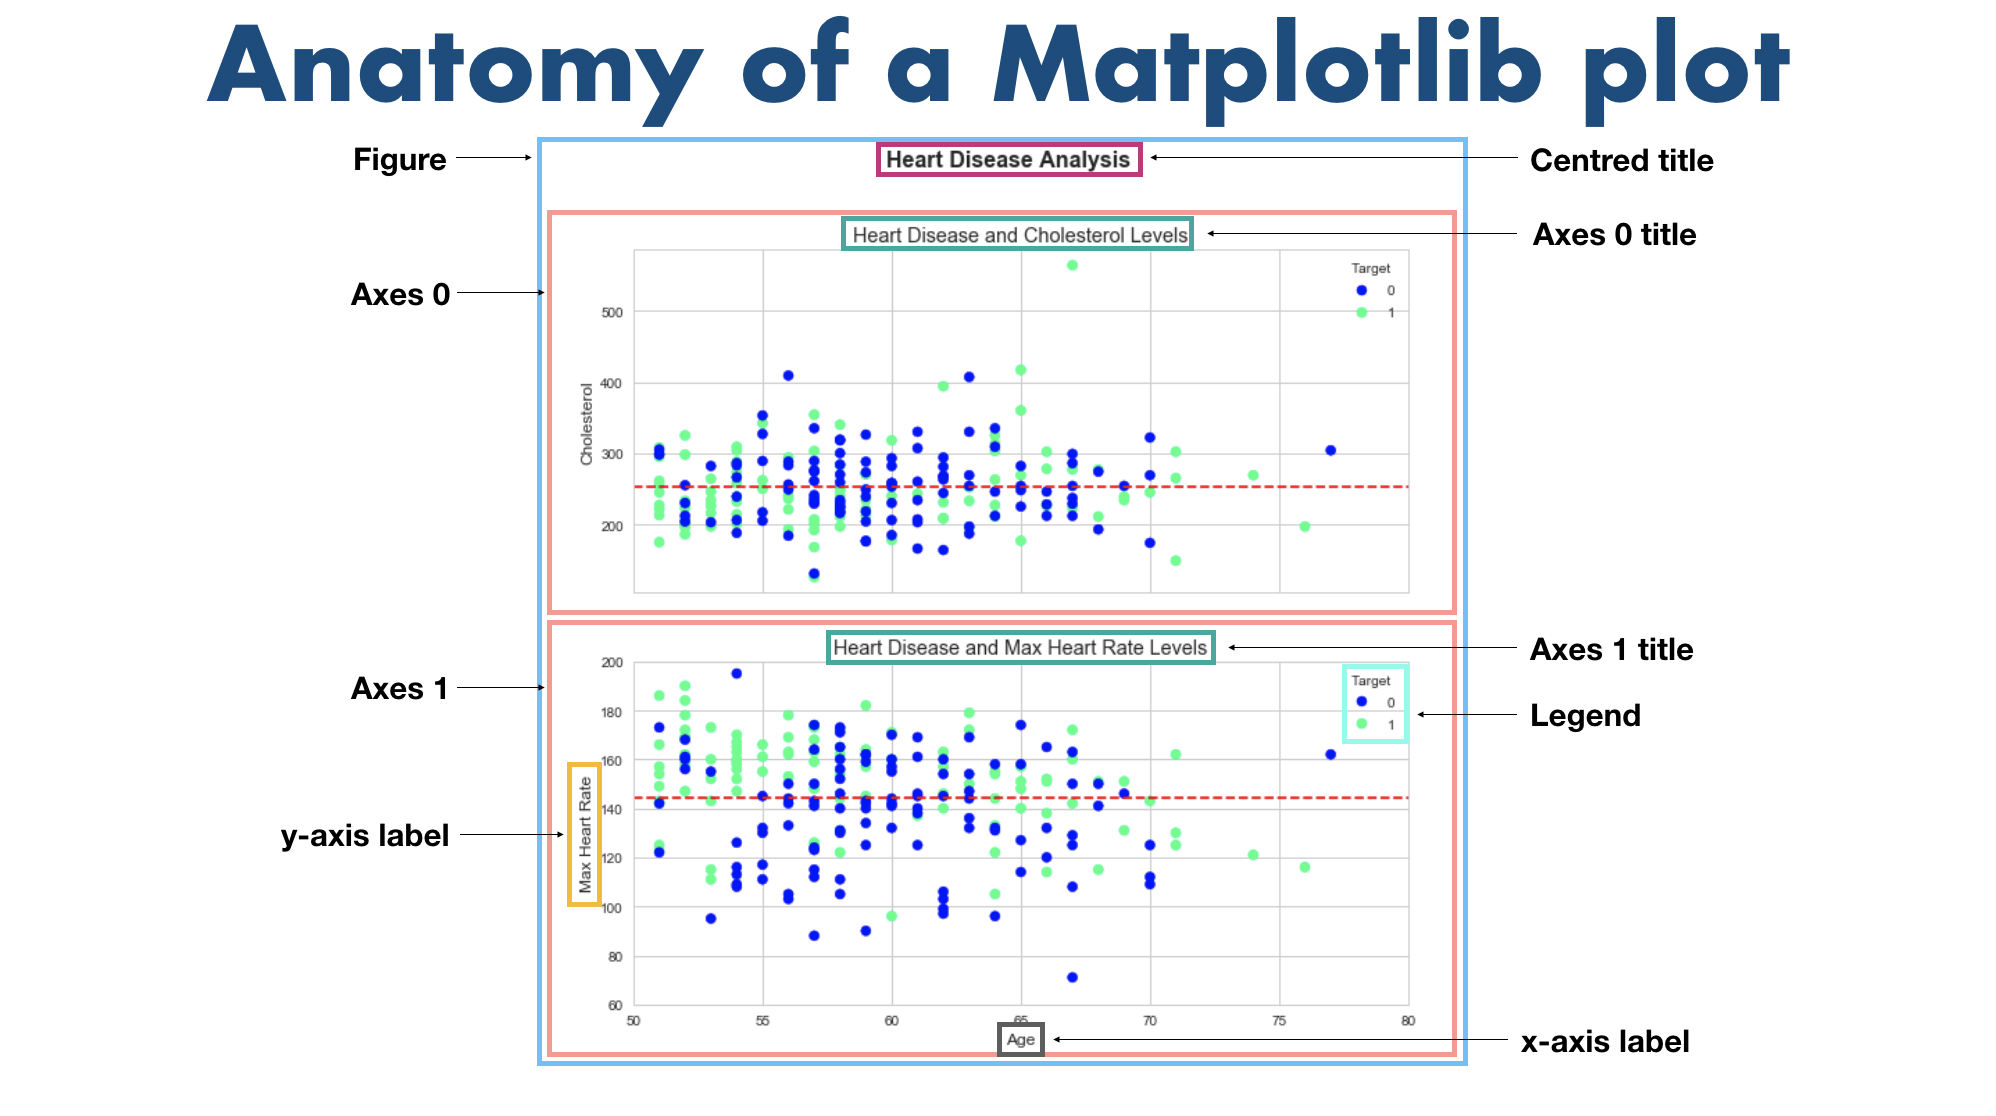
\includegraphics[scale=.5]{anatomy} \\
	We can create figures using data from NumPy arrays. Some common plot types we might use are:
	\begin{lstlisting}
	x = np.linespace(0, 10, 100) # 100 evenly spaced numbers between 0 and 10
	
	fig, ax = plt.subplots()
	
	ax.plot(x, x**2) # create a line graph 
	ax.scatter(x, np.exp(x)) # create a scatter plot
	ax.bar(['Almonds', 'Peanuts'], [10, 12]) # create a bar chart
	ax.hist(x) # create a histogram \end{lstlisting} \newpage
%%%% PAGE 9 %%%%

	\subsubsection{Subplots}
	We can create figures with subplots that can each contain different data or be different graph types. In order to access the subplots, we chose one of the following methods. If we pass in a tuple when creating the objects, we can access by calling a graph on the given object. If we create the objects without tuples, we must use indexing in order to access the graph at the position we want.  
	\begin{lstlisting}
	x = np.random.randn(1000)
	
	# Create a 10x5 figure with 4 subplots (2 in each row/column)
	fig, ((ax1, ax2), (ax3, ax4)) = plt.subplots(nrows = 2,
	                                             ncols = 2,
	                                             figsize = (10,5)) 
	# access sublots: ax1.plot(), ax2.hist(), etc.
	
	# Create a 10x5 figure with 4 subplots (2 in each row/column)
	fig, ax = plt.subplots(nrows = 2,
	                       ncols = 2,
	                       figsize = (10,5))                                            
	# access subplots: ax[0,0].plot(), ax[0,1].scatter(), etc. \end{lstlisting} \vspace*{1mm}
	
	\subsection{Plotting from Pandas DataFrames}                                             
	Before we begin to plot our data, we need to make sure that the columns are numeric. We can do this with \textit{regular expression (regex)}. We also may want to create new columns from data that already exist. Note that we can \textbf{plot directly} from a Pandas data frame using a built-in matplotlib method with the parameter \textit{kind=} to specify the type of graph we want. 
	\begin{lstlisting}
	car_sales = pd.read_csv('car-sales.csv')
	
	car_sales['Price'] = car_sales['Price'].str.replace('[\$\,\.]', '') # remove symbols
	car_sales['Price'] = car_sales['Price'].str[:-2] # remove extra zeros
	car_sales['Price'] = car_sales['Price'].astype(int) # cast as an integer
	
	# create a sale date column for each row in our data frame
	car_sales['Sale Date'] = pd.date_range('1/1/2020', periods = len(car_sales))
	
	# create total sales column by summing all prices
	car_sales['Total Sales'] = car_sales['Price'].cumsum()	
	
	car_sales.plot(x='Odometer (KM)', y='Price', kind='scatter')
	plt.show() \end{lstlisting} \vspace*{1mm}
	It is easy to use the built in plotting methods when creating simple graphs, but for creating more advanced plots we want to use the object-oriented API for matplotlib. Creating a figure and axes will allow us to add more features and variables to our plots.
	\begin{lstlisting}
	heart_disease = pd.read_csv('heart-disease.csv') 
	
	over_50 = heart_disease[heart_disease['age'] > 50]
	
	# create a scatter plot of age vs. chol, colored by the target values (OO Method)
	fig, ax = plt.subplots(figsize=(10, 6))
	scatter = ax.scatter(x=over_50['age'], y=over_50['chol'], c=over_50['target'])	
	
	ax.set(title='Heart Disease and Cholesterol Levels', xlabel='Age', 
	       ylabel='Cholesterol')       
	ax.legend(*scatter.legend_elements(), title='Target') # legend elements from 'c='
	
	ax.axhline(over_50['chol'].mean(), linestyle='--') \end{lstlisting} \newpage
%%%% PAGE 10 %%%%

	\noindent We can also create \textbf{subplots} directly from our Pandas data frames. By default, it uses the same scale and range for every subplot (which can start to look messy). Similar to above, we need to use the object-oriented API for creating subplots from axes objects. (note that the below code will output a similar graph to the `anatomy of a matplotlib plot' picture above). 
	\begin{lstlisting}
	fig, (ax0, ax1) = plt.subplots(nrows=2, ncols=1, figsize=(10,10))
	
	# Plot and customize axis 0 graph
	scatter = ax0.scatter(x=over_50['age'], y=over_50['chol'], c=over_50['target'])
	ax0.set(title='Heart Disease and Cholesterol Levels', xlabel='Age', 
	        ylabel='Cholesterol')
	ax0.legend(*scatter.legend_elements(), title='Target')      
	ax0.axhline(over_50['chol'].mean(), linestyle='--') # mean line
	
	# Plot and customize axis 1 graph
	scatter = ax1.scatter(x=over_50['age'], y=over_50['thalach'], c=over_50['target'])
	ax1.set(title='Heart Disease and Max Heart Rate', xlabel='Age', 
	        ylabel='Max Heart Rate')
	ax1.legend(*scatter.legend_elements(), title='Target')      
	ax1.axhline(over_50['thalach'].mean(), linestyle='--') # mean line 
	
	fig.suptitle('Heart Disease Analyis', fontsize=16, fontweight='bold') \end{lstlisting} \vspace*{1mm}
	
	\subsection{Customizing Plots}
	We can customize our plots to not only make them more visually appealing but also to more easily read the data from them. We can see all the available styles by using the \textit{plt.style.available} function. You want to run the \textit{plt.style.use()} method at the beginning of the notebook to make sure all graphs are the same style. Below we changed the graph from above and added: cmap, set\_xlim, set\_ylim.
	\begin{lstlisting}
	plt.style.use('seaborn-whitegrid') # change the style of our plot
	
	fig, (ax0, ax1) = plt.subplots(nrows=2, ncols=1, figsize=(10,10))
	
	# Plot and customize axis 0 graph
	scatter = ax0.scatter(x=over_50['age'], y=over_50['chol'], c=over_50['target'], 
	                      cmap='winter') # this changes the color scheme
	ax0.set(title='Heart Disease and Cholesterol Levels', xlabel='Age', 
	        ylabel='Cholesterol')
	ax0.set_xlim([50, 80]) # change the x-axis range limits
	ax0.set_ylim([60, 200]) # change the y-axis range limits
	ax0.legend(*scatter.legend_elements(), title='Target')      
	ax0.axhline(over_50['chol'].mean(), linestyle='--') # mean line
	
	# Plot and customize axis 1 graph
	scatter = ax1.scatter(x=over_50['age'], y=over_50['thalach'], c=over_50['target'],
	                      cmap='winter') # this changes the color scheme
	ax1.set(title='Heart Disease and Max Heart Rate', xlabel='Age', 
	        ylabel='Max Heart Rate')
	ax1.set_xlim([50, 80]) # change the x-axis range limits
	ax1.set_ylim([60, 200]) # change the y-axis range limits
	ax1.legend(*scatter.legend_elements(), title='Target')      
	ax1.axhline(over_50['thalach'].mean(), linestyle='--') # mean line 
	
	fig.suptitle('Heart Disease Analyis', fontsize=16, fontweight='bold')
	
	fig.savefig('Heart-disease-analysis.png') # saves to current directory \end{lstlisting} \newpage
%%%% PAGE 11 %%%%

	\section{Scikit-learn: Machine Leaning Models}
	\subsection{Workflow}
	We will follow a typical workflow when working with machine learning models. We will go over each step in detail, but this section is a general overview of how our it will look. We have the following steps: \\
	\hspace*{2mm} 1) Getting the data ready. \\
	\hspace*{2mm} 2) Choose the right estimator/algorithm for our problem. \\
	\hspace*{2mm} 3) Fit the model/algorithm and use it to make predictions on our data. \\
	\hspace*{2mm} 4) Evaluating a model. \\
	\hspace*{2mm} 5) Improve a model. \\
	\hspace*{2mm} 6) Save and load a trained model.	
	\begin{lstlisting}
	import pandas as pd
	import numpy as np
	
	# Step 1: getting data ready
	heart_disease = pd.read_csv('data/heart-disease.csv')
	X = heart_disease.drop('target', axis=1) # create features matrix
	y = heart_disease['target'] # create labels matrix
	
	# Step 2: Chose the model and hyperparameters
	from sklearn.ensemble import RandomForestClassifier
	clf = RandomForestClassifier(n_estimators = 100) 
	clf.get_params() # show the parameter values
	
	#Step 3: Fit the model to the training data
	from sklearn.model_selection import train_test_split
	X_train, X_test, y_train, y_test = train_test_split(X, y, test_size = 0.2)
	clf.fit(X_train, y_train) # find patterns in training data
	y_preds = clf.predict(X_test)
	
	# Step 4: Evaluate the model on training and test data
	clf.score(X_train, y_train) # 1.0
	clf.score(X_test, y_test) # 0.754
	
	from sklearn.metrics import classification report, confusion_matrix, accuracy_score
	classification_report(y_test, y_preds) # compare test labels to pred labels
	confusion_matrix(y_test, y_preds)
	accuracy_score(y_test, y_preds) # 0.754
	
	# Step 5: Improve the model
	np.random.seed(42)
	for i in range(10, 100, 10): 
		print(f'Trying model with {i} estimators...')
		clf = RandomForestClassifier(n_estimators = i).fit(X_train, y_train)
		print(f'Model accuracy on test set: {clf.score(X_test, y_test) * 100:.2f}%')
		print("") # after running loop, we see 20 estimators gets us to 83% accuracy
	
	# Step 6: Save model and load it
	import pickle
	
	pickle.dump(clf, open('random_forst_model_1.pkl', 'wb')) # saves to a file in dir
	
	loaded_model = pickle.load(open('random_forst_model_1.pkl', 'rb'))
	loaded_model.score(X_test, y_test)	\end{lstlisting} \newpage
%%%% PAGE 12 %%%%
	
	\subsection{Step 1: Getting Data Ready}
	There are three main things we must to when getting our data ready to be used in a ML model: \\
	\hspace*{2mm} 1) Split the data into features (X) and labels (y). \\
	\hspace*{2mm} 2) Filling (also called imputing) or disregarding missing values. \\
	\hspace*{2mm} 3) Converting non-numerical values to numerical values (called feature coding). \vspace*{2mm} \\
	Lets begin with \textbf{step 1}:
	\begin{lstlisting}
	heart_disease = pd.read_csv('heart-disease.csv')
	
	# Split into features and labels
	X = heart_disease.drop('target', axis=1)
	y = heart_disease['target']
	
	# Split into training and test sets
	from sklearn.model_selection import train_test_split
	X_train, X_test, y_train, y_test = train_test_split(X, y, test_size = 0.2) \end{lstlisting} \vspace*{1mm}
	Lets jump to \textbf{step 3}, where we want to \textbf{convert categorical to numerical data}. We will use a different data set as an example since our heart-disease.csv is already all numeric. Our `Make' column is categorical data with strings representing the values, so we need to convert these to numerical in order to use in our machine learning model. \\~\\
	\begin{minipage}[c]{9.3cm}
	One Hot Encoding is a process used to turn categories into numbers. It encodes values into 0's and 1's that allows us to feed it into a machine learning model. We can also do this is with the pd.get\_dummies( ) method, which does the same thing as OneHotEncoder.
	\end{minipage} 
	\begin{minipage}[c]{9cm}
	\hspace*{2mm} 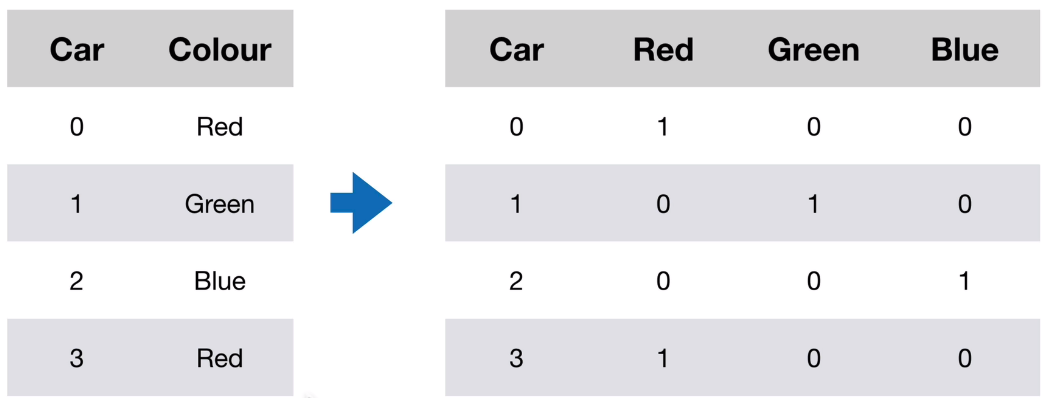
\includegraphics[scale=.28]{ohe}
	\end{minipage}
	\begin{lstlisting}
	np.random.seed(42)
	car_sales = pd.read_csv('car-sales-extended.csv')
	
	X = car_sales.drop['Price', axis=1]
	y = car_sales['Price']
		
	# Convert categorical to numerical data
	from sklearn.preprocessing import OneHotEncoder
	from sklearn.compose import ColumnTransformer
	
	# Option 1: One Hot Encoder method
	categorical_features = ['Make', 'Colour', 'Doors']
	one_hot = OneHotEncoder()
	transformer = ColumnTransformer([('one_hot', one_hot, categorical_features)], 
	                                remainder='passthrough')
	transformed_X = transformer.fit_transform(X)
	
	# Option 2: Pandas get_dummies() method
	dummies = pd.get_dummies(car_sales[['Make', 'Colour', 'Doors']])
	
	# Fit the model with the new data
	X_train, X_test, y_train, y_test = train_test_split(transformed_X, y, 
	                                                    test_size = 0.2)
	
	from sklearn.ensemble import RandomForestRegressor # predicts numbers
	model = RandomForestRegressor()
	model.fit(X_train, y_train)
	model.score(X_test, y_test)	# .3043 (not much data for each sample)\end{lstlisting} \newpage
%%%% PAGE 13 %%%%

	\noindent For \textbf{step 2}, there are two main ways of dealing with missing data: \\
	\hspace*{2mm} 1) Fill them with some value (also known as imputation). \\
	\hspace*{2mm} 2) Remove the samples with missing data altogether. \vspace*{1.5mm} \\
	Before we can convert our data into numerical values, we must drop or fill the NaN values. Lets look at the first option, which is \textbf{filling the missing data with Pandas}. We want to drop any samples that do not have a label since we don't want to try and predict them ourselves.
	\begin{lstlisting}
	car_sales_missing = pd.read_csv('data/car-sales-extended-missing-data.csv') 
	
	car_sales_missing.isna().sum() # around 50 values missing in each column
	
	################ Fill in missing values using Pandas ################
	car_sales_missing['Make'].fillna('missing', inplace=True)
	car_sales_missing['Colour'].fillna('missing', inplace=True)
	car_sales_missing['Odometer (KM)'].fillna(car_sales_missing['Odometer (KM)'].mean(), 
	                                          inplace=True)
	car_sales_missing['Doors'].fillna(4, inplace=True)
	car_sales_missing.dropna(inplace=True) # drop missing values in Price column
	
	# Split data and concert to numerical
	X = car_sales_missing.drop['Price', axis=1]
	y = car_sales_missing['Price']
	
	categorical_features = ['Make', 'Colour', 'Doors']
	one_hot = OneHotEncoder()
	transformer = ColumnTransformer([('one_hot', one_hot, categorical_features)], 
	remainder='passthrough')
	transformed_X = transformer.fit_transform(X) \end{lstlisting} \vspace*{1mm}
	Our second option for missing values is to \textbf{fill NaN values with scikit-learn}. An important note is that you want to split your train/test data before filling missing values so that you don't use test data to fill training data (and vice versa). 
	\begin{lstlisting}
	car_sales_missing = pd.read_csv('data/car-sales-extended-missing-data.csv') 	
	
	car_sales_missing.dropna(subset=['Price'], inplace=True) # drop rows with no labels
	X = car_sales_missing.drop['Price', axis=1]
	y = car_sales_missing['Price']
	
	# Split into train/test data before filling missing values
	np.random.seed(42)
	X_train, X_test, y_train, y_test = train_test_split(X, y, test_size=0.2)
	
	############### Fill missing values using scikit-learn ###############
	from sklearn.impute import SimpleImputer
	from sklearn.compose import ColumnTransformer
	
	# Fill categorical values with 'missing' & numerical values with mean
	cat_imputer = SimpleImputer(strategy="constant", fill_value="missing") # categorical
	door_imputer = SimpleImputer(strategy="constant", fill_value=4) # door column
	num_imputer = SimpleImputer(strategy="mean") # numerical
	
	cat_features = ["Make", "Colour"]
	door_feature = ["Doors"]
	num_features = ["Odometer (KM)"]
	
	# Create an imputer (something that fills missing data)
	imputer = ColumnTransformer([
		("cat_imputer", cat_imputer, cat_features), # (name, imputer, features)
		("door_imputer", door_imputer, door_feature),
		("num_imputer", num_imputer, num_features) ]) 
		
	# Fill train and test values separately
	filled_X_train = imputer.fit_transform(X_train)
	filled_X_test = imputer.transform(X_test)
	
	# Get our transformed data array's back into DataFrame's
	car_sales_filled_train = pd.DataFrame(filled_X_train, 
	                                      columns=["Make", "Colour", "Doors", 
	                                               "Odometer (KM)"])
	
	car_sales_filled_test = pd.DataFrame(filled_X_test, 
	                                     columns=["Make", "Colour", "Doors", 
	                                              "Odometer (KM)"])
	
	# Use OneHotEncoder to encode the data
	categorical_features = ["Make", "Colour", "Doors"]
	one_hot = OneHotEncoder()
	transformer = ColumnTransformer([("one_hot", one_hot, categorical_features)],
	                                remainder="passthrough")
	
	# Fill train and test values separately
	transformed_X_train = transformer.fit_transform(car_sales_filled_train)
	transformed_X_test = transformer.transform(car_sales_filled_test)
	
	np.random.seed(42)
	from sklearn.ensemble import RandomForestRegressor
	
	model = RandomForestRegressor(n_estimators=100)
	model.fit(transformed_X_train, y_train)
	model.score(transformed_X_test, y_test) # 0.2123 (lower score due to less samples) \end{lstlisting} \vspace*{1mm}
	
	\subsection{Step 2: Choosing the Right Model}
	Scikit-learn uses \textbf{estimator} as another term for machine learning model or algorithm. There are two different types of estimators we will focus on: \\
	\hspace*{2mm} 1) Classification - predicting whether a sample is one thing or another. \\
	\hspace*{2mm} 2) Regression - predicting a number value. \\
	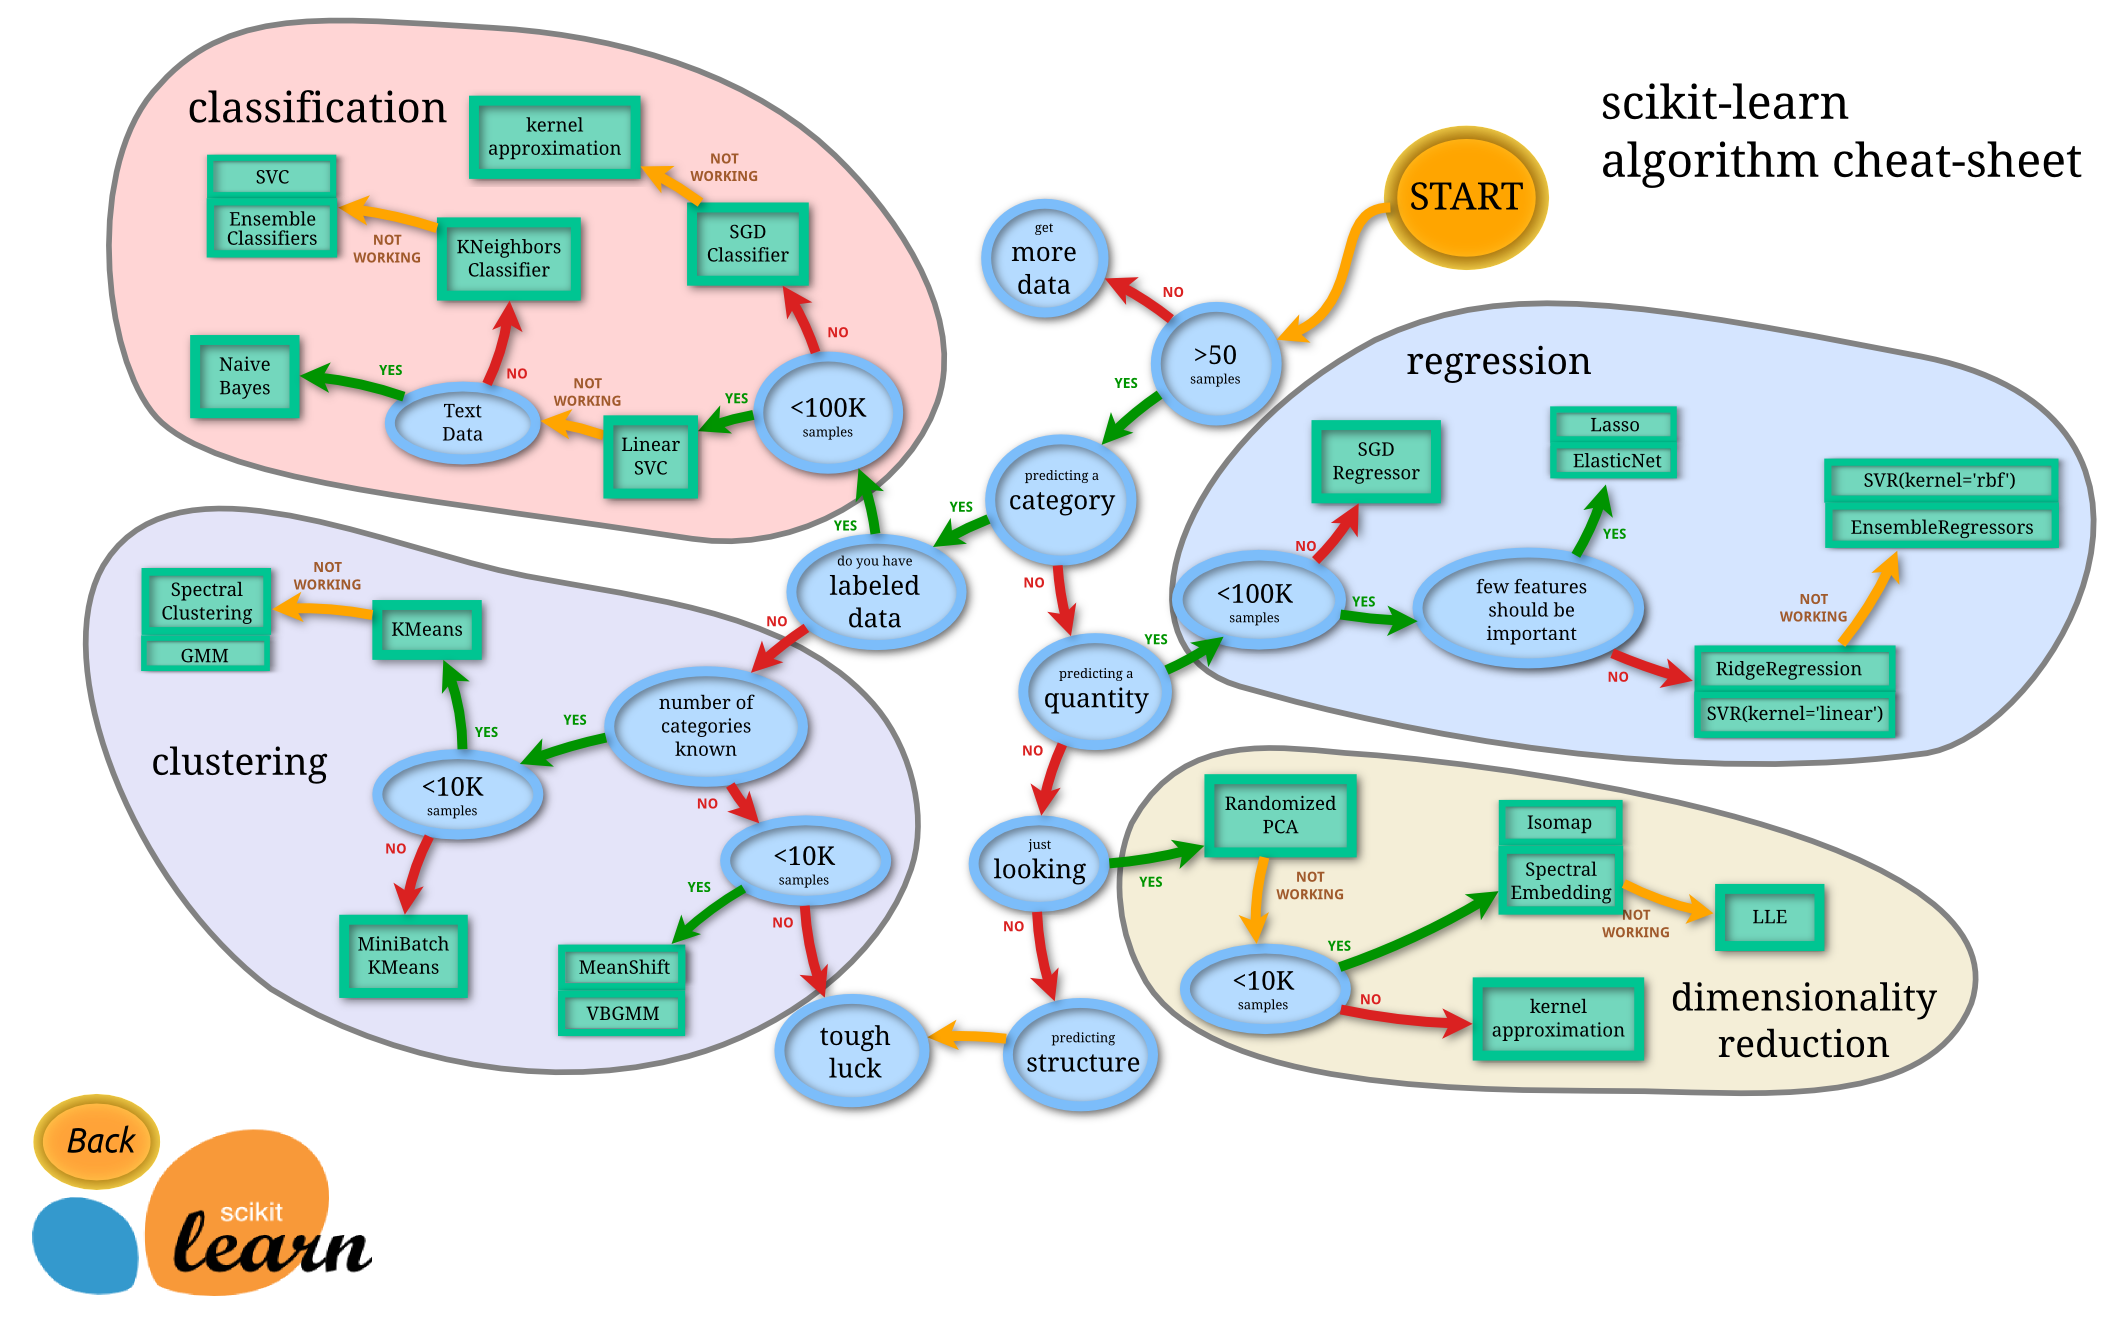
\includegraphics[scale=.11]{est} \\
	\href{https://scikit-learn.org/stable/tutorial/machine_learning_map/index.html}{Click here} for the link to the picture (all green boxes are clickable). \newpage
%%%% PAGE 15 %%%%

	\subsubsection{Regression models}
	We will use the dataset within the scikit-learn library that contains information on \href{https://scikit-learn.org/stable/datasets/index.html}{housing in Boston}. Looking at the picture above, we have over 50 samples and we want to predict a quantity. We also have less than 100k samples and more than a few features are important, so we will use \textit{RidgeRegression}. 
	\begin{lstlisting}
	from sklearn.datasets import load_boston
	from sklearn.linear_model import Ridge
	np.random.seed(42)
	
	boston = load_boston() # loads in as a dictionary
	boston_df = pd.DataFrame(boston['data'], columns=boston['feature_names'])
	boston_df['target'] = pd.Series(boston['target'])
	len(boston_df) # 506 samples
	
	X = boston_df.drop('target', axis=1)
	y = boston_df['target']
	
	X_train, X_test, y_train, y_test = train_test_split(X, y, test_size=0.2)
	
	model = Ridge()
	model.fit(X_train, y_train)
	model.score(X_test, y_test) # R^2 = 0.6662 \end{lstlisting} \vspace*{1mm}
	From this point, our Ridge model is currently working. But what if it wasn't? Also, how can we improve our $R^2$ score for the model? If the model wasn't working, we can use \textbf{ensemble regressors}, which use several base estimators to improve over a single estimator. One example of this method is by using the \textit{RandomForestRegressor}. We will use the train/test data from above.
	\begin{lstlisting}
	from sklearn.ensemble import RandomForestRegressor
	np.random.seed(42)
	
	rf = RandomForestRegressor(n_estimators = 100)
	rf.fit(X_train, y_train)
	rf.score(X_test, y_test) # R^2 = 0.87397 \end{lstlisting} \vspace*{1mm}
	
	\subsubsection{Classification models}
	We will use the heart-disease.csv to classify whether or not someone has heart disease. We have more than 50 samples and we are predicting a category. We have labeled data and less than 100k samples, so we want to use a \textit{LinearSVC} classifier (we find this by looking at the image map above).
	\begin{lstlisting}
	from sklearn.svm import LinearSVC
	np.random.seed(42)
	
	heart_disease = pd.read_csv('data/heart-disease.csv') 
	
	X = heart_disease.drop('target', axis=1)
	y = heart_disease['target']
	
	X_train, X_test, y_train, y_test = train_test_split(X, y, test_size=0.2)
	
	clf = LinearSVC(max_iter=10000)
	clf.fit(X_test, y_test)
	clf.score(X_test, y_test) # 0.4754 \end{lstlisting} \vspace*{1mm}
	This is a binary classification problem, and our model in only at a 47\% accuracy. This is not good since there are only two classes, so if we were to guess we would only get half of them correct (this could mean the model isn't finding all of the patterns). Looking at the image above, we see that we want to use \textbf{ensemble classifiers} in order to improve our score. \newpage
%%%% PAGE 16 %%%%
	
	\begin{lstlisting}
	from sklearn.ensemble import RandomForestClassifier
	np.random.seed(42)
	
	clf = RandomForestClassifier(n_estimators = 100)
	clf.fit(X_train, y_train)
	clf.score(X_test, y_test) # R^2 = 0.85246 \end{lstlisting} \vspace*{1mm}
	The key takeaway from this section is that if you have \textbf{structured data}, use ensemble methods as the estimator. The Random Forest is known for its robustness and ability to have a high $R^2$ score. If you have \textbf{unstructured data}, use deep/transfer learning.
	\subsection{Step 3: Making Predictions with our Model}
	\textbf{Classification:} \vspace*{1mm} \\
	There are two ways to use a trained model to make predictions. One way is with the \textbf{.predict( )} function. This will return an array of labels, one for each sample/row, which we can then compare to the truth labels (y\_test). We will use the RandomForestClassifier model from above as our trained estimator. 
	\begin{lstlisting}
	# Compare predictions to truth labels to evalaute the model
	y_preds = clf.predict(X_test)
	np.mean(y_preds == y_test) # 0.85246 \end{lstlisting} \vspace*{1mm}
	The second way we can make predictions is with the \textbf{.predict\_proba( )} function. This will return an array of probabilities for each classification label (ordered by the label of classes). The label with the largest probability will be the class for which the model assigns the prediction. 
	\begin{lstlisting}
	clf.predict_proba(X_test) # first value in array is [0.89, 0.11]
	clf.predict(X_test) # first value is 0 (since label 0 had larger probability) \end{lstlisting} \vspace*{1mm}
	\textbf{Regression:} \vspace*{1mm} \\
	The scikit-learn .predict( ) method can also be used on regression models. We can then compare the predictions to the truth using mean\_absolute\_error, which takes the difference between the prediction and truth and takes the average of them all (plus/minus value).
	\begin{lstlisting}
	X = boston_df.drop('target', axis=1)
	y = boston_df['target']
	X_train, X_test, y_train, y_test = train_test_split(X, y, test_size=0.2)
	
	model = RandomForestRegressor(n_estimators = 100).fit(X_train, y_train)
	y_preds = model.predict(X_test)
	
	from sklearn.metrics import mean_absolute_error
	mean_absolute_error(y_test, y_preds) # 2.12 away for target \end{lstlisting} \vspace*{1mm}
	
	\subsection{Step 4: Evaluating a Model}
	There are 3 different ways to evaluate a scikit-learn model/estimator: \\
	\hspace*{2mm} 1) Estimator `score' method. \\
	\hspace*{2mm} 2) The `scoring' parameter. \\
	\hspace*{2mm} 3) Problem-specific metric functions. \vspace*{2mm} \\
	We will begin with the \textbf{score method}. The score() function has a default evaluation metric built in to it. For \textit{regression}, it will use the coefficient of determination ($R^2$). For \textit{classification}, it returns the mean accuracy on the data that is passed in. \newpage
%%%% PAGE 17 %%%%

	\begin{lstlisting}
	from sklearn.ensemble import RandomForestClassifier
	np.random.seed(42)
	
	X = heart_disease.drop('target', axis=1)
	y = heart_disease['target']
	X_train, X_test, y_train, y_test = train_test_split(X, y, test_size=0.2)
	
	clf = RandomForestClassifier(n_estimators = 100).fit(X_train, y_train)
	clf.score(X_test, y_test) # 0.852459
	\end{lstlisting} \vspace*{1mm}
	Next we will look at the \textbf{scoring parameter}. We can use a \textbf{cross validation} method, which splits the data into `k' different splits and is evaluated on each one. Note that we pass X and y into the function, not the test data splits. It avoids getting lucky high scores by training and evaluating on all of the data. We can then take the average of the scores to find our value. \vspace*{1mm} \\
	Note that if the \textit{scoring=} parameter is set to None, it will use the default scoring parameter of our estimator ($R^2$ for regression and \textit{mean accuracy} for classification). 
	\begin{lstlisting}
	from sklearn.model_selection import cross_val_score
	np.random.seed(42)
	
	clf_cross_val_score = np.mean(cross_val_score(clf, X, y, cv=5)) # 0.8248 \end{lstlisting} \vspace*{1mm}
	\subsubsection{Evaluating a Classification Model}
	There are 4 main evaluation metrics that we can use for classification models: accuracy, area under ROC curve, confusion matrix, and classification report. \vspace*{1.5mm} \\
	Lets begin with the \textbf{accuracy} evaluation metric: 
	\begin{lstlisting}
	from sklearn.model_selection import cross_val_score
	from sklearn.ensemble import RandomForestClassifier	
	np.random.seed(42)
	
	X = heart_disease.drop('target', axis=1)
	y = heart_disease['target']
	
	clf = RandomForestClassifier(n_estimators = 100)
	c_v_score = cross_val_score(clf, X, y, cv=5)
	np.mean(c_v_score) # 0.8248	\end{lstlisting} \vspace*{1mm}
	Next, lets look at the area under the receiver operating characteristic curve (\textbf{AUC/ROC}). ROC curves are a comparison of a model's true positive rate (tpr) vs a models false positive rate (fpr). \\
	\hspace*{2mm} - True positive: model predicts 1 when truth is 1. \\
	\hspace*{2mm} - False positive: model predicts 1 when truth is 0. \\
	\hspace*{2mm} - True negative: model predicts 0 when truth is 0. \\
	\hspace*{2mm} - False negative: model predicts 0 when truth is 1.
	\begin{lstlisting}
	from sklearn.metrics import roc_curve
	
	X_train, X_test, y_train, y_test = train_test_split(X, y, test_size=0.2)
	
	clf = RandomForestClassifier(n_estimators = 100).fit(X_test, y_test)
	y_probs = clf.predict_proba(X_test)
	
	y_probs_positive = y_probs[:, 1] # only keep columns with 1's probability \end{lstlisting} \newpage
%%%% PAGE 18 %%%%
	
	\begin{lstlisting}
	fpr, tpr, threshold = roc_curve(y_test, y_probs_positive)
	
	def plot_roc_curve(fpr, tpr):
		plt.plot(fpr, tpr, color='orange', label='ROC') # roc curve
		plt.plot([0,1], [0,1], color='darkblue', linestyle='--', label='Guessing') # base
		plt.xlabel('False Positive Rate (FPR)')
		plt.ylabel('True Positive Rate (TPR)')
		plt.title('Receiver Operating Characteristic (ROC) Curve')
		plt.legend()
		plt.show()
	
	plot_roc_curve(fpr, tpr) 
	
	from sklearn.metrics import roc_auc_score
	roc_auc_score(y_test, y_probs_positive) # 0.84967 \end{lstlisting} \vspace*{1mm}
	A \textbf{confusion matrix} is a quick way to compare the labels a model predicts and the actual labels it was supposed to predict. In essence, it gives you an idea of where the model is getting `confused'. \vspace*{1mm}\\ It is easiest to visualize a confusion matrix with the \textit{pd.crosstab( )} function, but we can also get more advanced with Seaborn's \textit{heatmap()} function.
	\begin{lstlisting}
	from sklearn.metrics import confusion_matrix
	
	y_preds = clf.predict(X_test)
	conf_mat = confusion_matrix(y_test, y_preds)
	# create a table which shows true pos/neg and false pos/neg results
	pd.crosstab(y_test, y_preds, rownames=['Actual Label'], colnames=['Predicted Label'])
	
	import seaborn as sns
	
	def plot_conf_mat(conf_mat):
		fig, ax = plt.subplots(figsize=(3,3))
		ax = sns.heatmap(conf_mat, annot=True, cbar=False)
		plt.xlabel('True Label')
		plt.ylabel('Predicted Label')
		plt.show() \end{lstlisting} \vspace*{1mm}
	The final evaluation metric is a \textbf{classification report}. It is a collection of the following metrics: \\
	\hspace*{2mm} - Precision : proportion of positive identifications (1) that were correct. \\
	\hspace*{2mm} - Recall : proportion of actual positives that were correctly classified. \\
	\hspace*{2mm} - F1 score : combination of recall and precision (want a score near 1.0). \\
	\hspace*{2mm} - Support : the number of samples each metric was calculated on. \\
	\hspace*{2mm} - Accuracy : the percent of correct predictions. \\
	\hspace*{2mm} - Macro average : average of precision, recall, and F1 score between classes (watch for class imbalance). \\
	\hspace*{2mm} - Weighted Average : same as macro average, but with respect to number of samples. \vspace*{1mm} \\
	Note that for data with \textit{class imbalances} (more samples in one class than another), you want to use a metric other than just accuracy. 
	\begin{lstlisting}
	from sklearn.metrics import classification_report
	
	classification_report(y_test, y_preds) \end{lstlisting} \vspace*{1mm}
	Classification metrics summary: \\
	\hspace*{2mm} - \textbf{Accuracy} is good to start with if all classes are balanced.\\
	\hspace*{2mm} - \textbf{Precision/Recall} become more important when there is a class imbalance. \\
	\hspace*{2mm} - If false positive predictions are worse than false negatives, aim for higher precision. \\
	\hspace*{2mm} - If false negative predictions are worse than false positives, aim for higher recall. \\
	\hspace*{2mm} - \textbf{F1-score} is a combination of precision and recall. \newpage
%%%% PAGE 19 %%%%
	
	\subsubsection{Evaluating a Regression Model}
	There are 3 main model evaluation metrics that we will focus on: $R^2$ (coefficient of determination), MAE (mean absolute error), and MSE (mean squared error). First lets set up a regression model to evaluate.
	\begin{lstlisting}
	import sklearn.ensemble import RandomForestRegressor
	np.random.seed(42)
	
	X = boston_df.drop('target', axis=1)
	y = boston_df['target']
	X_train, X_test, y_train, y_test = train_test_split(X, y, test_size=0.2)
	
	model = RandomForestRegressor(n_estimators = 100).fit(X_train, y_train)	\end{lstlisting} \vspace*{1mm}
	$\mathbf{R^2}$ is the default return value from the .score( ) method. This compares your models prediction to the mean of the target. Values can range from negative infinity to 1. If your model predicts the mean every time, it will have a value of 0. But if your model perfectly predicts a range of numbers it's $R^2$ value would be 1.
	\begin{lstlisting}
	from sklearn.metrics import r2_score
	
	mode.score(X_test, y_test) # 0.87387
	
	# create an array of y_test mean values to compare of predictions
	y_test_mean = np.full(len(y_test), y_test.mean()) 
	
	r2_score(y_test, y_test_mean) # 0.0
	r2_score(y_test, y_test) # 1.0	\end{lstlisting} \vspace*{1mm}
	Now lets take a look at \textbf{MAE} (mean absolute error). This is the average of the absolute value of the difference between predicted and actual values. It gives you an idea of how wrong your models prediction are on average (plus/minus the given value from the actual value). 
	\begin{lstlisting}
	from sklearn.metrics import mean_absolute_error
	
	y_preds = model.predict(X_test)
	mae = mean_absolute_error(y_test, y_preds) # 2.12 \end{lstlisting} \vspace*{1mm}
	Finally lets look at \textbf{MSE} (mean squared error). This will always be higher than MAE because it squares the errors. It squares the difference between predicted and actual values, then takes the mean value.	
	\begin{lstlisting}
	from sklearn.metrics import mean_squared_error
	
	mse = mean_squared_error(y_test, y_preds) # 9.242 \end{lstlisting} \vspace*{1mm}
	Which regression metric should you use? You want to minimize MSE and MAE while maximizing the $R^2$ value. \\
	\hspace*{2mm} - $\mathbf{R^2}$ is similar to accuracy. It gives you a quick indication but doesn't tell you how wrong your model \hspace*{4mm} is in terms of difference for each prediction. \\
	\hspace*{2mm} - \textbf{MAE} gives better indication of how fart off each of your models prediction are on average. \\
	\hspace*{2mm} - \textbf{MSE} will amplify larger differences.
	
	\subsubsection{Cross Validation and Scoring parameter}
	By default the cross validation method uses the default scoring parameter: for classification this is \textit{mean accuracy}, and for regression this is the $R^2$ value. Note that for regression, the MSE and MAE are negative since as the value gets larger (moves from negative to positive) it means are model is performing better. In the future, it could be helpful to write a function that will neatly output these metrics for the user. \newpage
%%%% PAGE 20 %%%%

	\begin{lstlisting}
	from sklearn.model_selection import cross_val_score
	from sklearn.ensemble import RandomForestClassifier
	from sklearn.ensemble import RandomForestRegressor
	np.random.seed(42)
	
	# Classification model scoring
	X = heart_disease.drop('target', axis=1)
	y = heart_disease['target']
	clf = RandomForestClassifier(n_estimators = 100)
	
	cv_acc = cross_val_score(clf, X, y, cv=5) 
	cv_precision =  cross_val_score(clf, X, y, cv=5, scoring='precision') 
	cv_recall = cross_val_score(clf, X, y, cv=5, scoring='recall')
	cv_f1 = cross_val_score(clf, X, y, cv=5, scoring='f1')
	
	# Regression model scoring
	X = boston_df.drop('target', axis=1)
	y = boston_df['target']
	model = RandomForestRegressor(n_estimators = 100)
	
	cv_r2 = cross_val_score(model, X, y, cv=5) 
	cv_mae = cross_val_score(model, X, y, cv=5, scoring='neg_mean_absolute_error') 
	cv_mse = cross_val_score(model, X, y, cv=5, scoring='neg_mean_squared_error') \end{lstlisting} \vspace*{1mm}
	\subsubsection{Metric Functions with scikit-learn}
	Lets begin with classification evaluation functions:
	\begin{lstlisting}
	from sklearn.metrics import accuracy_score, precision_score, recall_score, f1_score
	from sklearn.ensemble import RandomForestClassifier
	from sklearn.model_selection import train_test_split
	np.random.seed(42)
	
	X = heart_disease.drop('target', axis=1)
	y = heart_disease['target']
	X_train, X_test, y_train, y_test = train_test_split(X, y, test_size=0.2)
	clf = RandomForestClassifier(n_estimators = 100).fit(X_train, y_train)
	
	y_preds = clf.predict(X_test)
	accuracy_score(y_test, y_preds) # 0.8525
	precision_score(y_test, y_preds) # 0.8484
	recall_score(y_test, y_preds) # 0.875
	f1_score(y_test, y_preds) # 0.8615	\end{lstlisting} \vspace*{1mm}
	Next, lets look at regression evaluation functions:
	\begin{lstlisting}
	from sklearn.metrics import r2_score, mean_absolute_error, mean_squared_error
	from sklearn.ensemble import RandomForestRegressor
	from sklearn.model_selection import train_test_split
	np.random.seed(42)
	
	X = boston_df.drop('target', axis=1)
	y = boston_df['target']
	X_train, X_test, y_train, y_test = train_test_split(X, y, test_size=0.2)
	model = RandomForestRegressor(n_estimators = 100).fit(X_train, y_train)
	
	y_preds = model.predict(X_test)
	r2_score(y_test, y_preds) # 0.8739
	mean_absolute_error(y_test, y_preds) # 2.122
	mean_squared_error(y_test, y_preds) # 9.24 \end{lstlisting} \newpage
%%%% PAGE 21 %%%%

	\subsection{Step 5: Improving a Model}
	The first predictions you make are the \textbf{baseline predictions}. The first model you build is the \textbf{baseline model}. We want to focus on how to improve both of these in two different ways. \vspace*{1mm} \\
	The first is from a data perspective: \\
	\hspace*{2mm} 1) Could we collect more data? (generally the more data, the better). \\
	\hspace*{2mm} 2) Could we improve our data? \vspace*{1mm} \\
	The second is from a model perspective: \\
	\hspace*{2mm} 1) Is there a better model? (moving from simple to complex models). \\
	\hspace*{2mm} 2) Could we improve the current model? (hyperparameters). \vspace*{1mm} \\
	The difference between parameters and hyperparameters are that \textbf{parameters} are patterns in data that are model will find, while \textbf{hyperparameters} are settings on a model that we can adjust to \textit{potentially} improve its ability to find patterns. \vspace*{2mm} \\ 
	We can use the .get\_params() method to see the hyperparameters that we are able to adjust.
	\begin{lstlisting}
	from sklearn.ensemble import RandomForestClassifier

	clf = RandomForestClassifier()
	clf.get_params()	\end{lstlisting} \vspace*{1mm}
	There are \textbf{three ways to adjust hyperparameters} that will will look at: manually by hand, randomly with RandomizedSearchCV, and exhaustively with GridSearchCV. 
	\subsubsection{Tuning Hyperparameters Manually}
	When tuning hyperparameters, we will us the \textbf{validation set} (10-15\% of the data). Lets begin by writing a function that will print evaluation metrics from a \textit{classification} model:
	\begin{lstlisting}
	def evaluate_preds(y_true, y_preds):
		accuracy = accuracy_score(y_true, y_preds)
		precision = precision_score(y_true, y_preds)
		recall = recall_score(y_true, y_preds)
		f1 = f1_score(y_true, y_preds)
		metric_dict = {'accuracy': round(accuracy, 2),
		               'precision': round(precision, 2),
		               'recall': round(recall, 2),
		               'f1': round(f1, 2) }
		print('Acc: {}'.format(accuracy * 100:0.2f))              
		print('Precision: {}'.format(precision:0.2f))
		print('Recall: {}'.format(recall:.2f))
		print('F1 Score: {}'.format(f1:0.2f))
		return metric_dict \end{lstlisting} \vspace*{1mm}
	Next lets split the data into training, validation, and test split (by hand):
	\begin{lstlisting}
	from sklearn.ensemble import RandomForestClassifier
	np.random.seed(42)
	
	heart_disease_shuffled = heart_disease.sample(frac=1)
	X = heart_disease_shuffled.drop('target', axis=1)
	y = heart_disease_shuffled['target']
	
	train_split = round(0.7 * len(heart_disease_shuffled)) # 70% of data
	valid_split = round(train_split + 0.15 * len(heart_disease_shuffled)) # 15% of data
	X_train, y_train = X[:train_split], y[:train_split]
	X_valid, y_valid = X[train_split:valid_split], y[train_split:valid_split]
	X_test, y_test = X[valid_split:], y[valid_split:] \end{lstlisting} \newpage
%%%% PAGE 22 %%%%

	\noindent We can now use these splits to see how our model is performing and tune any hyperparameters:
	\begin{lstlisting}
	clf = RandomForestClassifier()
	clf.fit(X_train, y_train)
	y_preds = clf.predict(X_valid) # baseline predictions
	baseline_metrics = evaluate_preds(y_valid, y_preds) # 80%, 0.77, 0.92, 0.84
	
	# Create a second classifier with different hyperparameters & make predictions
	clf_2 = RandomForestClassifier(n_estimators=100)
	clf_2.fit(X_train, y_train)
	y_preds_2 = clf_2.predict(X_valid)
	clf_2_metrics = evaluate_preds(y_valid, y_preds_2) # 82.2%, 0.84, 0.84, 0.84
	# we see a slight boost in accuracy, higher precision, lower recall, same f1 \end{lstlisting} \vspace*{1mm}
	\subsubsection{Tuning Hyperparameters with RandomizedSearchCV}
	We can tune hyperparameters using \textbf{RandomizedSearchCV}. We will create a dictionary of the hyperparameters we want to tune with the parameter as the key and the value as the parameter values we want to try. We don't need a validation set since we will use a k-fold cross validation. The model below will test 50 different combinations (5 cv sets for 10 different models).
	\begin{lstlisting}
	from sklearn.model_selection import RandomizedSearchCV 
	np.random.seed(42)
	
	grid = {'n_estimators': [10, 100, 200, 500, 1000, 1200],
	        'max_depth': [None, 5, 10, 20, 30],
	        'max_features': ['auto', 'sqrt'],
	        'min_samples_split': [2, 4, 6],
	        'min_samples_leaf': [1, 2, 4]}
	
	X = heart_disease_shuffled.drop('target', axis=1)
	y = heart_disease_shuffled['target']
	X_train, X_test, y_train, y_test = train_test_split(X, y, test_size=0.2) 
	clf = RandomForestClassifier(n_jobs=1) # n_jobs is dedicated CPU power    
	
	# Setup RandomizedSearchCV
	rs_clf = RandomizedSearchCV(estimator=clf, 
	                            param_distributions=grid, 
	                            n_iter=10, # number of models to try
	                            cv=5, # creates 5 different validation sets
	                            verbose=2)	
	                            
	# Fit the RandomizedSearchCV version of clf
	rs_clf.fit(X_train, y_train)
	rs_clf.best_params_ # shows which combination got best results
	
	# Make predictions with best hyperparameters & evaluate
	rs_y_preds = rs_clf.predict(X_test)
	rs_metrics = evaluate_preds(y_test, rs_y_preds) # 81.97%, 0.77, 0.86, 0.81 \end{lstlisting} \vspace*{1mm}
	\subsubsection{Tuning Hyperparameters with GridSearchCV}
	For \textbf{GridSearchCV}, it will try every single combination that is possible from our grid. Since we know what the best hyperparameters are for our model from the previous RandomizedSearchCV, we can use those to influence which ones we will keep when shrinking the search space in our new grid. We now will only test 60 different models (3*1*2*1*2 choices in our grid multiplied by 5 cv gives us 60 models). \newpage
%%%% PAGE 23 %%%%
	
	\begin{lstlisting}
	from sklearn.model_selection import GridSearchCV, train_test_split
	np.random.seed(42)
	
	grid_2 = {'n_estimators': [100, 200, 500],
	          'max_depth': [None],
	          'max_features': ['auto', 'sqrt'],
	          'min_samples_split': [6],
	          'min_samples_leaf': [1, 2]}
	
	# Use the data splits and original clf model from previous code block
	# Setup GridSearchCV
	gs_clf = RandomizedSearchCV(estimator=clf, 
	                            param_grid=grid_2, 
	                            cv=5,
	                            verbose=2)	
	
	# Fit the GridSearchCV version of clf
	gs_clf.fit(X_train, y_train)
	gs_clf.best_params_
	
	gs_y_preds = gs_clf.predict(X_test)
	gs_metrics = evaluate_preds(y_test, gs_y_preds) # 78.7%, 0.74, 0.82, 0.78 \end{lstlisting} \vspace*{1mm}
	The final step is to compare the different models metrics.
	\begin{lstlisting}
	compare_metrics = pd.DataFrame({'baseline': baseline_metrics,
	                                'clf_2': clf_2_metrics,
	                                'random search': rs_metrics,
	                                'grid search': gs_metrics}) 
	                                
	compare_metrics.plot.bar(figsize=(10,8)); \end{lstlisting} \vspace*{1mm}
	\subsection{Step 6: Saving and Loading a Model}
	After we train and tune a model, we might want to save it so that we can use it outside of our Jupyter Notebook. There are two different ways in which we can save a model: with Python's `pickle' module, or with the 'joblib' module. 
	\begin{lstlisting}
	import pickle
	
	# Save model in our current working directory using Pickle
	pickle.dump(gs_clf, open('gs_random_random_forest_model_1.pkl', 'wb')) 
	
	# Load saved model
	loaded_pickle_model = pickle.load(open('gs_random_random_forest_model_1.pkl', 'rb'))
	
	# Make predictions using model
	pickle_y_preds = loaded_pickle_model.predict(X_test)
	evaluate_preds(y_test, pickle_y_preds)	\end{lstlisting} \vspace*{1mm}
	\begin{lstlisting}
	from joblib import dump, load
	
	dump(gs_clf, filename='gs_random_forest_model_1.joblib') # save a joblib model
	
	loaded_job_model = load(filename='gs_random_forest_model_1.joblib') # load in model
	
	# Make and evaluate joblib predictions
	joblib_y_preds = loaded_job_model.predict(X_test)
	evaluate_preds(y_test, joblib_y_preds) \end{lstlisting} \newpage
%%%% PAGE 24/25 %%%%

	\subsection{Putting It All Together}
	We will use the \textbf{scikit-learn Pipeline} class as a way to string together a bunch of scikit processes in one hit (similar to a function). In one cell block, we want to: fill missing data, convert it to numeric, and build a model on the data. 
	\begin{lstlisting}	
	# Modules for getting data ready
	import pandas as pd
	from sklearn.compose import ColumnTransformer
	from sklearn.pipeline import Pipeline
	from sklearn.impute import SimpleImputer
	from sklearn.preprocessing import OneHotEncoder
	
	# Modelling tools
	from sklearn.ensemle import RandomForestRegressor
	from sklearn.model_selection import train_test_split, GridSearchCV
	
	# Setup random seed
	import numpy as np
	np.random.seed(42)
	
	# Import data and drop rows with missing labels
	data = pd.read_csv('data/car-sales-extended-missing-data.csv')
	data.dropna(subset=['Price'], inplace=True)
	
	# Define different features and transformer pipeline
	categorical_features = ['Make', 'Color']
	categorical_transformer = Pipeline(steps=[
		('imputer', SimpleImputer(strategy='constant', fill_value='missing')),
		('onehot', OneHotEncoder(handle_unknown='ignore'))]) # turn data into numbers
	
	door_feature = ['Doors']
	door_transformer = Pipeline(steps=[
		('imputer', SimpleImputer(strategy='constant', fill_value='4'))])
	
	numeric_features = ['Odometer (KM)']
	numeric_transformer = Pipeline(steps=[
		('imputer', SimpleImputer(strategy='mean'))])
	
	# Setup preprocessing steps (fill missing values and convert to numeric)
	preprocessor = ColumnTransformer(
	                    transformer=[
	                    	('cat', categorical_transformer, categorical_features),
	                    	('door', door_transformer, door_feature),
	                    	('num', numeric_transformer, numeric_features) ])
	
	# Create a preprocessing and modelling pipeline
	model = Pipeline(steps=[('preprocessor', preprocessor), 
	                        ('model', RandomForestRegressor()) ])
	
	# Split data
	X = data.drop('Price', axis=1)
	y = data['Price'] 
	X_train, X_test, y_train, y_test = train_test_split(X, y, test_size=0.2)
	
	# Fit and score the model
	model.fit(X_train, y_train)
	model.score(X_test, y_test) # 0.1822 \end{lstlisting} \vspace*{1mm}
	Now that we have trained our mode, we can use GridSearchCV or RandomizedSearchCV with our Pipeline to tune the hyperparameters to try and improve our models score. \newpage
%%%% PAGE 25 %%%%

	\noindent The double underscore in the pipe\_grid below is used as an accessor. We can think of it as the first value being the step name in the Pipeline we want to access, and following values being the step action within the Pipeline to look for that we want to change.
	\begin{lstlisting}
	# Use GridSearchCV with our regression Pipeline
	from sklearn.model_selection import GridSearchCV
	
	pipe_grid = {
		'preprocessor__num__imputer__strategy': ['mean', 'median'],
		'model__n_estimators': [100, 1000],	
		'model__max_depth': [None, 5],
		'model__max_features': ['auto'], # 'model' step, change max_features of model
		'model__min_samples_split': [2, 4]
	} # 16 different combinations of parameters
	
	gs_model = GridSearchCV(model, pipe_grid, cv=5, verbose=2) # 16*5 = 80 models
	gs_model.fit(X_train, y_train) 
	
	gs_model.score(X_test, y_test) # 0.3338 (double the original model score) \end{lstlisting} \vspace*{2mm}
	
	\subsection{Milestone Project 1 (Classification)}
	We will use the heart disease dataset for this project. Following the typical work flow that we covered in section one, lets map out our data modeling steps. \vspace*{1.5mm} \\
	\textbf{Step 1: Problem Definition} \\
	Given clinical parameters about a patient, can we predict whether or not they have heart disease? \vspace*{1.5mm} \\
	\textbf{Step 2: Data} \\
	The original data came from the Cleveland data from the \href{https://archive.ics.uci.edu/ml/datasets/heart+Disease}{UCI Machine Learning Repository}.There is also a version of it available on \href{https://www.kaggle.com/ronitf/heart-disease-uci}{Kaggle}. \vspace*{1.5mm} \\
	\textbf{Step 3: Evaluation} \\
	If we can reach 95\% accuracy at predicting whether or not a patient has heart disease during the proof of concept, we'll pursue the project. \vspace*{1.5mm} \\
	\textbf{Step 4: Features} \\
	This is where you'll get different information about each of the features in your data. We can look at the link above for the UCI Irvine repository to see a description of the 14 features that are within our dataset. \vspace*{1.5mm} \\
	\textbf{Import Tools}	
	\begin{lstlisting}
	# Regular EDA (exploratory data analysis) and plotting libraries
	import numpy as np
	import pandas as pd
	import matplotlib.pyplot as plt
	import seaborn as sns
	
	# Models and Evaluations from Scikit-Learn
	from sklearn.linear_model import LogisticRegression
	from sklearn.neighbors import KNeighborsClassifier
	from sklearn.ensemble import RandomForestClassifier
	
	from sklearn.model_selection import train_test_split, cross_val_score
	from sklearn.model_selection import RandomizedSearchCV, GridSearchCV
	from sklearn.metrics import confusion_matrix, classification_report
	from sklearn.metrics import precision_score, recall_score, f1_score
	from sklearn.metrics import plot_roc_curve \end{lstlisting} \newpage
%%%% PAGE 26 %%%%

	\subsubsection{Data Exploration (EDA)}
	The goal here is to find out more about the data and become a subject matter export on the dataset. \\
	1. What question(s) are you trying to solve? \\
	2. What kind of data do we have and how do we treat different types? \\
	3. What's missing from the data and how do you deal with it? \\
	4. Where are the outliers and why should you care about them? \\
	5. How can you add, change or remove features to get more out of your data?
	\begin{lstlisting}
	df = pd.read_csv("../data/heart-disease.csv") # data folder from previous dir
	df.shape # (303, 14)
	df["target"].value_counts() # 1 (165), 0 (138). Even distribution
	df.info() # show data types, number of rpws/cols, etc.
	df.isna().sum() # find any missing values in each column
	df.describe() # get numerical analysis for each column	
	
	# Compare target column to the sex column
	df.sex.value_count() # 1 (207 males), 0 (96 females)
	pd.crosstab(df.target, df.sex).plot(kind="bar",	figsize=(10, 6),
	                                    color=["salmon", "lightblue"])
	plt.title("Heart Disease Frequency for Sex")
	plt.xlabel("0 = No Diesease, 1 = Disease")
	plt.ylabel("Amount")
	plt.legend(["Female", "Male"]);
	plt.xticks(rotation=0); \end{lstlisting} \vspace*{1mm}
	\begin{minipage}[c]{9cm}
	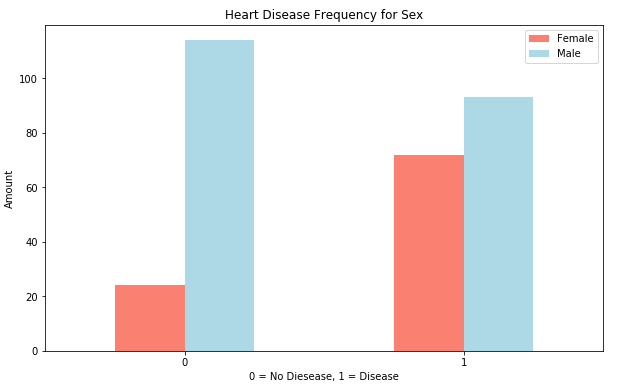
\includegraphics[scale=.5]{crosstab_hd}
	\end{minipage}
	\begin{minipage}[c]{8cm}
	We can see that for our graph, females have about a 75\% chance of having heart disease in our data set. For males, they have around a 50\% of having heart disease. We also know that there are about twice as many males than females in our data set as well.
	\end{minipage}
	\begin{lstlisting}
	# Compare age column against max heart rate column for heart disease
	plt.figure(figsize=(10,6))
	# create scatter plot of age vs max heart rate (positive for heart disease)
	plt.scatter(df.age[df.target==1], df.thalach[df.target==1], c='salmon')
	# create scatter plot of age vs max heart rate (negative for heart disease)
	plt.scatter(df.age[df.target==0], df.thalach[df.target==0], c='salmon')
	plt.title("Heart Disease in function of Age and Max Heart Rate")
	plt.xlabel("Age")
	plt.ylabel("Max Heart Rate")
	plt.legend(["Disease", "No Disease"]); \end{lstlisting} \vspace*{1mm}
	\begin{minipage}[c]{9cm}
	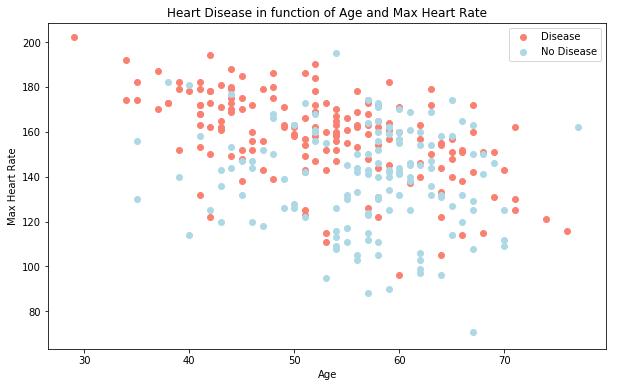
\includegraphics[scale=.5]{scatt_hd}
	\end{minipage}
	\begin{minipage}[c]{8cm}
	All we can see is a downward trend for both target values. As age increases, the maximum heart rate decreases in the individual. There is no real stand out pattern here, but it is a good analysis for understanding the data. 
	\end{minipage} \newpage
%%%% PAGE 27 %%%%

	\begin{lstlisting}
	# Does chest pain (cp) correlate to having heart disease?
	### note that chest pain can have 4 different values (0, 1, 2, 3) see UCI for details
	
	pd.crosstab(df.cp, df.target).plot(kind='bar', figsize=(10,6), 
	                                   color=['salmon', 'lightblue'])
	plt.title("Heart Disease Frequency Per Chest Pain Type")
	plt.xlabel("Chest Pain Type")
	plt.ylabel("Amount")
	plt.legend(["No Disease", "Disease"])
	plt.xticks(rotation=0);	\end{lstlisting} \vspace*{1mm}
	\begin{minipage}[c]{9cm}
	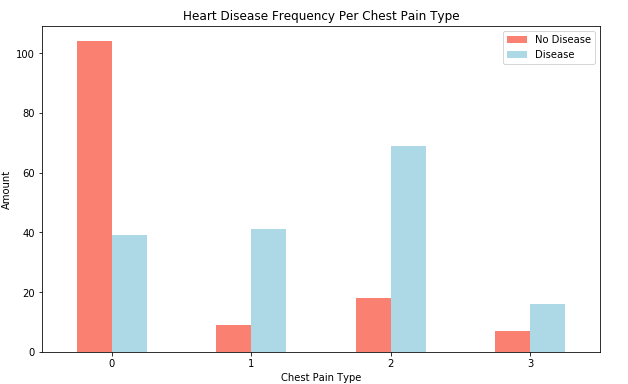
\includegraphics[scale=.5]{bar_hd}
	\end{minipage}
	\begin{minipage}[c]{8cm}
	An interesting find is that for heart disease 1 and 2 (which are both suppose to be not related to the heart), we see that they both have very high numbers for the patients who have this chest pain and have a target value of 1. 
	\end{minipage} \vspace*{1mm} \\
	We want to build a \href{https://www.displayr.com/what-is-a-correlation-matrix/#:~:text=A\%20correlation\%20matrix\%20is\%20a,a\%20diagnostic\%20for\%20advanced\%20analyses.}{correlation matrix} to tell us how related the independent variables are to one another. To make the visualization nicer, we can make a heatmap of our correlation matrix. 
	\begin{lstlisting}
	corr_matrix = df.corr()
	fig, ax = plt.subplots(figsize=(15, 10))
	ax = sns.heatmap(corr_matrix, annot=True, 
	                 linewidths=0.5, fmt=".2f", cmap="YlGnBu");
	bottom, top = ax.get_ylim() # get current limit values
	ax.set_ylim(bottom + 0.5, top - 0.5) # fix first/last row cut off \end{lstlisting} \vspace*{1mm}
	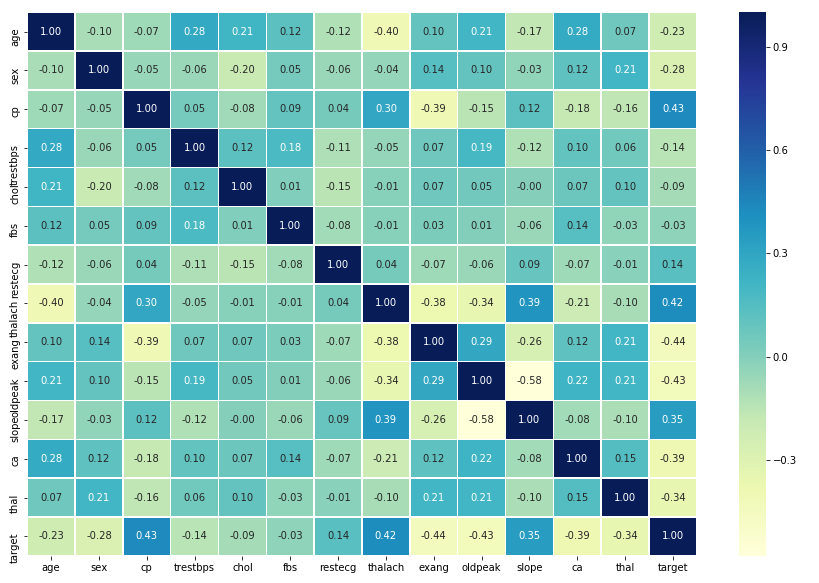
\includegraphics[scale=.75]{heat_hd} \newpage
%%%% PAGE 28 %%%%

	\subsubsection{Modeling (Step 5)}
	Before we begin modeling, we must split the data into training and test sets. 
	\begin{lstlisting}
	np.random.seed(42) # reproducible results
	
	X = df.drop('target', axis=1)
	y = df['target']
	X_train, X_test, y_train, y_test = train_test_split(X, y, test_size=0.2) \end{lstlisting} \vspace*{1mm}
	Referring back to the picture in section 5.3, we can see that KNeighborsClassifier and a RandomForestClassifier are the ideal choices. However, we will also include a LogisticRegression model since it is made for classification (not regression). The easiest way to test these models will be to put them in a dictionary, write a function to train/test them, and finally compare the scores for each model.
	\begin{lstlisting}
	models = {"Logistic Regression": LogisticRegression(),
	          "KNN": KNeighborsClassifier(),
	          "Random Forest": RandomForestClassifier()}
	
	def fit_and_score(models, X_train, X_test, y_train, y_test):
		"""
		Fits and evaluates given machine learning models.
		models : a dict of different Scikit-Learn machine learning models
		"""
		np.random.seed(42) # Set random seed
		model_scores = {} # Make a dictionary to keep model scores
		for name, model in models.items():
			model.fit(X_train, y_train) # Fit the model to the data
			model_scores[name] = model.score(X_test, y_test) # Evaluate append score
		return model_scores
	
	model_scores = fit_and_score(models, X_train, X_test, y_train, y_test)
	"""
	{'Logistic Regression': 0.8852459016393442,
	 'KNN': 0.6885245901639344,
	 'Random Forest': 0.8360655737704918}
	"""	\end{lstlisting} \vspace*{1mm}
	\subsubsection{Tuning Hyperparameters}
	Our KNN classifier was our lowest score in the previous subsection, so lets see if we can improve this score by tuning the hyperparameters by hand.
	\begin{lstlisting}
	train_scores = []
	test_scores = []
	
	neighbors = range(1, 21) # Create a list of differnt values for n_neighbors
	knn = KNeighborsClassifier() # Setup KNN instance
	
	for i in neighbors: # Loop through different n_neighbors
		knn.set_params(n_neighbors=i) # Set n_neighbors value
		knn.fit(X_train, y_train) # Fit the algorithm
		train_scores.append(knn.score(X_train, y_train)) # Update the training scores list
		test_scores.append(knn.score(X_test, y_test)) # Update the test scores list
	
	plt.plot(neighbors, train_scores, label="Train score")
	plt.plot(neighbors, test_scores, label="Test score")
	plt.xticks(np.arange(1, 21, 1))
	plt.xlabel("Number of neighbors")
	plt.ylabel("Model score")
	plt.legend()
	print(f"Maximum KNN score on the test data: {max(test_scores)*100:.2f}%")	\end{lstlisting} \vspace*{1mm}
	\begin{minipage}[c]{9cm}
	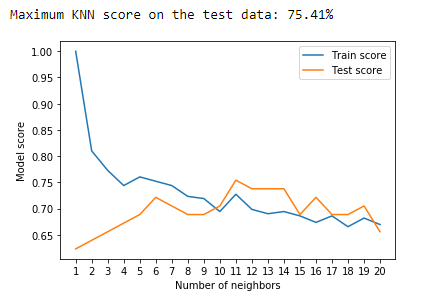
\includegraphics[scale=.8]{knn_mp}
	\end{minipage}
	\begin{minipage}[c]{8cm}
	We can see that a n\_neighbor value of 11 gives us the highest score on the test data. We were able to go from 68.8\% to 75.4\% by only tuning one hyperparameter. However, even with the tuning it still has a lower score than LogisticRegression or the RandomForestClassifier. Because of this, we will discard the model and focus mainly on the other two. 
	\end{minipage} \vspace*{4mm} \\
	Now we will tune the LogisticRegression and RandomForestClassifier models with RandomizedSearchCV. 
	\begin{lstlisting}
	# Create a hyperparameter grid for LogisticRegression model
	log_reg_grid = {"C": np.logspace(-4, 4, 20),
	                "solver": ["liblinear"]}
	
	# Create a hyperparameter grid for RandomForestClassifier model
	rf_grid = {"n_estimators": np.arange(10, 1000, 50),
	           "max_depth": [None, 3, 5, 10],
	           "min_samples_split": np.arange(2, 20, 2),
	           "min_samples_leaf": np.arange(1, 20, 2)}
	
	############################# Tune LogisticRegression #############################
	np.random.seed(42)
	
	# Setup random hyperparameter search for LogisticRegression
	rs_log_reg = RandomizedSearchCV(LogisticRegression(), # model to use
	                                param_distributions=log_reg_grid, # hyper grid
	                                cv=5, # 5 different data set splits
	                                n_iter=20, # 20 different models
	                                verbose=True) # 100 different fits
	
	rs_log_reg.fit(X_train, y_train) # Fit random hyperparameter search model
	
	rs_log_reg.best_params_ # {'solver': 'liblinear', 'C': 0.23357214690901212}
	rs_log_reg.score(X_test, y_test) # 0.8852 (no increase in score)
	
	########################### Tune RandomForestClassifier ###########################
	np.random.seed(42)
	
	# Setup random hyperparameter search for RandomForestClassifier
	rs_rf = RandomizedSearchCV(RandomForestClassifier(), # model to use
	                           param_distributions=rf_grid, # hyper grid
	                           cv=5, # 5 different data set splits
	                           n_iter=20, # 20 different models
	                           verbose=True) # 100 different fits
	
	rs_rf.fit(X_train, y_train) # Fit random hyperparameter search model 
	
	rs_rf.best_params_ # {'n_estimators': 210, 'min_samples_split': 4, 
	                   #  'min_samples_leaf': 19, 'max_depth': 3}
	rs_rf.score(X_test, y_test) # 0.8688 (increase of 0.032) \end{lstlisting} \newpage
%%%% PAGE 30 %%%%

	\noindent After the results above, the LogisticRegression model has the higher score and we will focus on that one. Now that we have used RandomizedSearchCV (which chooses hyperparameters from our grid at random), we will use GridSearchCV with our model (which exhaustively tries all combinations within our hyperparameter grid). 
	\begin{lstlisting}
	# Different hyperparameters for our LogisticRegression model
	log_reg_grid = {"C": np.logspace(-4, 4, 30),
	                "solver": ["liblinear"]}
	                
	# Setup grid hyperparameter search for LogisticRegression
	gs_log_reg = GridSearchCV(LogisticRegression(),
	                          param_grid=log_reg_grid, # 30 different combinations
	                          cv=5, # 5 different data splits
	                          verbose=True) # 150 total fits
	
	gs_log_reg.fit(X_train, y_train) # Fit grid hyperparameter search model
	
	gs_log_reg.best_params_ # {'C': 0.20433597178569418, 'solver': 'liblinear'}
	gs_log_reg.score(X_test, y_test) # 0.8852 (again no increase) \end{lstlisting} \vspace*{1mm}
	\subsubsection{Evaluating the Model}
	We want to evaluate our model beyond just accuracy. The first metric we want to see is a \textbf{ROC curve}, which is the true positive rate plotted against the false positive rate (we can use the sklearn built in function for this). A perfect ROC curve would get an AUC score of 1. 
	\begin{lstlisting}
	y_preds = gs_log_reg.predict(X_test) # Make predictions with tuned model
	
	# Plot ROC curve and calculate and calculate AUC metric
	plot_roc_curve(gs_log_reg, X_test, y_test) \end{lstlisting} \vspace*{1mm}
	Next we want to see a \textbf{confusion matrix}, but we can use a heatmap to make it more easily readable.
	\begin{lstlisting}
	sns.set(font_scale=1.5)
	
	def plot_conf_mat(y_test, y_preds):
		fig, ax = plt.subplots(figsize=(3, 3))
		ax = sns.heatmap(confusion_matrix(y_test, y_preds),	annot=True, 	cbar=False)
		plt.xlabel("True label")
		plt.ylabel("Predicted label")
		
		bottom, top = ax.get_ylim()
		ax.set_ylim(bottom + 0.5, top - 0.5)
	
	plot_conf_mat(y_test, y_preds) \end{lstlisting} \vspace*{1mm}
	Below are the visualizations for the above code (ROC curve on left, confusion matrix on right): \\
	\begin{minipage}[c]{9cm}
	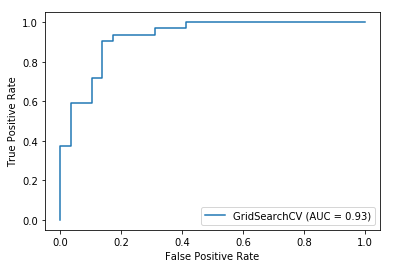
\includegraphics[scale=.8]{roc_mp}
	\end{minipage}
	\begin{minipage}[c]{8cm}
	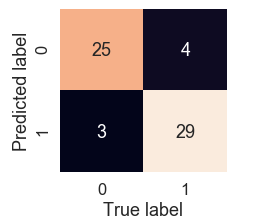
\includegraphics[scale=.8]{conf_mat_mp}
	\end{minipage} \newpage
%%%% PAGE 31 %%%%
	
	\noindent Now we will look at a \textbf{classification report}, which gives us precision, recall, and f1 score. \\
	\hspace*{3mm} - \textit{Precision} : indicates the proportion of positive (1) predictions that were actually correct. \\
	\hspace*{3mm} - \textit{Recall} : indicates the proportion of actual positives (1) that were correctly classified. \\
	\hspace*{3mm} - \textit{f1} : a combination of recall and precision (should be near or equal to 1).
	\begin{lstlisting}
	classification_report(y_test, y_preds)
	#     precision   recall   f1-score
	# 0   0.89        0.86     0.88
	# 1   0.88        0.91     0.89
	# accuracy                 0.89 \end{lstlisting} \vspace*{1mm}
	Note that this report is only used on the original data split. We need to use \textbf{cross validation} to find k-fold cross validation scores for all of the metrics listed in the classification report. We will need to create a new LogisticRegression model that is not already trained on data (but use the best hyperparameters found earlier). 
	\begin{lstlisting}
	# Create a new classifier with best parameters
	gs_log_reg.best_params_ # {'C': 0.20433597178569418, 'solver': 'liblinear'}
	clf = LogisticRegression(C=0.20433597178569418,	solver="liblinear")
	
	# Cross-validated accuracy
	cv_acc = cross_val_score(clf, X, y, cv=5, scoring="accuracy")
	np.mean(cv_acc) # 0.8446994535519124
	
	# Cross-validated precision
	cv_precision = cross_val_score(clf, X, y, cv=5, scoring="precision")
	np.mean(cv_precision) # 0.8207936507936507
	
	# Cross-validated recall
	cv_recall = cross_val_score(clf, X, y, cv=5, scoring="recall")
	np.mean(cv_recall) # 0.9212121212121213
	
	# Cross-validated f1-score
	cv_f1 = cross_val_score(clf, X, y, cv=5, scoring="f1")
	np.mean(cv_f1) # 0.8673007976269721
	
	# Visualize cross-validated metrics
	cv_metrics = pd.DataFrame({"Accuracy": cv_acc, "Precision": cv_precision,
	                           "Recall": cv_recall, "F1": cv_f1}, index=[0])
	
	cv_metrics.T.plot.bar(title="Cross-validated classification metrics", legend=False); \end{lstlisting} \vspace*{1mm}
	\begin{minipage}[c]{9cm}
	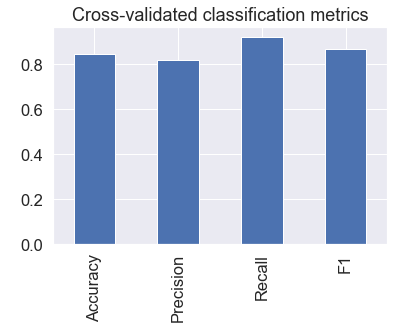
\includegraphics[scale=.8]{cv_mp}
	\end{minipage}
	\begin{minipage}[c]{8cm}
	We see that our recall (the proportion of positive class (1) values were correctly predicted) is the highest score in our cross validation evaluation. In the future, it would be helpful to turn the above code into a function that would output the scores and create a graph to visualize them. 
	\end{minipage} \newpage
%%%% PAGE 32 %%%%

	\subsubsection{Find Most Important Features}
	\textbf{Feature importance} is finding which features contributed most to the outcomes of the model and how did they contribute. For our model, which characteristics contribute most to heart disease? Note that finding this is different for each machine learning model (search for ``\textit{model name}'' feature importance). 
	\begin{lstlisting}
	# Fit an instance of LogisticRegression (with the best hyperparameters from earlier)
	clf = LogisticRegression(C=0.20433597178569418,	solver="liblinear")
	clf.fit(X_train, y_train)
	
	clf.coef_ # only used for LogisticRegression
	# [[ 0.00316727, -0.86044582,  0.66067073, -0.01156993, -0.00166374,
	#    0.04386131,  0.31275787,  0.02459361, -0.60413038, -0.56862852,
	#    0.45051617, -0.63609863, -0.67663375]]
	
	# Match coef's of features to columns from data frame (into an dict)
	feature_dict = dict(zip(df.columns, list(clf.coef_[0])))
	
	# Visualize feature importance
	feature_df = pd.DataFrame(feature_dict, index=[0])
	feature_df.T.plot.bar(title="Feature Importance", legend=False); \end{lstlisting} \vspace*{1mm}
	\begin{minipage}[c]{9cm}
	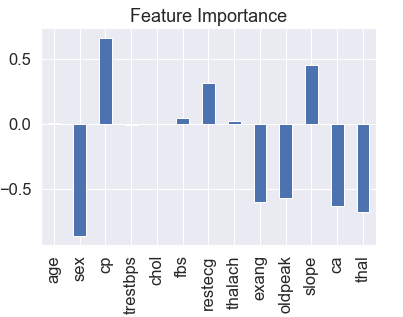
\includegraphics[scale=.8]{feat_mp}
	\end{minipage}
	\begin{minipage}[c]{8cm}
	We can see how much each of these independent variables contribute to finding the target variable. For example, as the value for sex increases then the ratio value for target decrease (since it is a negative correlation). It goes from a 3:1 ratio to a 1:2 ratio. For slope, as it increases so should the target value ratio.
	\end{minipage} \vspace*{1mm} \\
	\begin{minipage}[c]{9cm}
	\begin{lstlisting}
	pd.crosstab(df["sex"], df["target"])
	pd.crosstab(df["slope"], df["target"]) \end{lstlisting} \vspace*{1mm}
	\end{minipage}
	\begin{minipage}[c]{8cm}
	\hspace*{5mm} 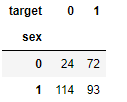
\includegraphics[scale=.8]{crosstab1_mp} \hspace*{2mm}
	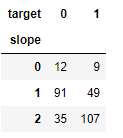
\includegraphics[scale=.8]{crosstab2_mp}
	\end{minipage} \vspace*{7mm} \\
	\textbf{Step 6: Experimentation} \\
	If you haven't hit your evaluation metric yet, ask yourself: \vspace*{1mm} \\	
	\hspace*{2mm} - Could you collect more data? \\
	\hspace*{2mm} - Could you try a better model? Like CatBoost or XGBoost? \\
	\hspace*{2mm} - Could you improve the current models? (beyond what we've done so far) \\
	\hspace*{2mm} - If your model is good enough (you have hit your evaluation metric) how would you export it and \hspace*{5mm} share it with others? \vspace*{3mm} \\
	NOTE: Search for ```classification dataset" to find new data that you can use for machine learning models. \newpage
%%%% PAGE 33 %%%%

	\subsection{Milestone Project 2 (Regression)}
	This is a \textbf{time series data set}, meaning that we will be using sales from the past to predict sales for the future. The data is split into 3 parts: Train.csv (data until end of 2011), Valid.csv (Jan-Apr 2012), Test.csv (May - Nov 2012). \\~\\
	
	
	
	
	
	
	
	
	
	
	
	
	
	
		
	\end{spacing}
\end{document}